% =====================================================================
%  BÁO CÁO MINI-PROJECT — TỐI ƯU LẬP KẾ HOẠCH
%  Đánh giá các phương pháp giải chính xác và metaheuristic
%  cho bài toán xếp thời khóa biểu.
%  Góc nhìn: NHÀ THIẾT KẾ GIẢI PHÁP (vấn đề -> lựa chọn -> đánh đổi -> bằng chứng).
%  Biên dịch: tectonic main.tex   (XeTeX, hỗ trợ Unicode tiếng Việt)
% =====================================================================
\documentclass[11pt,a4paper]{article}

\usepackage{fontspec}
\setmainfont{Times New Roman}
\usepackage{geometry}
\geometry{margin=2.4cm}
\usepackage{amsmath,amssymb,amsthm}
\usepackage{mathtools}
\usepackage{graphicx}
\usepackage{float}            % cho [H]: ảnh đặt ĐÚNG vị trí, không trôi
\usepackage{booktabs}
\usepackage{array}
\usepackage{multirow}
\usepackage{xcolor}
\usepackage{enumitem}
\usepackage{caption}
\usepackage{subcaption}
\usepackage[ruled,vlined,linesnumbered]{algorithm2e}
\usepackage{tikz}
\usetikzlibrary{positioning,arrows.meta,shapes.geometric,fit,backgrounds,calc}
\usepackage{titlesec}
\usepackage[hidelinks]{hyperref}
\usepackage{fancyhdr}
\usepackage{multirow}
\usepackage{tocloft}
% Tiêu đề mục lục: "Mục lục", căn giữa.
\renewcommand{\contentsname}{Mục lục}
\renewcommand{\cfttoctitlefont}{\hfill\color{accent}\Large\bfseries}
\renewcommand{\cftaftertoctitle}{\hfill}

\captionsetup{font=small,labelfont=bf}
\setlist{itemsep=2pt,topsep=3pt}

\definecolor{accent}{HTML}{1F4E79}
\definecolor{soft}{HTML}{EAF0F7}
\definecolor{cexact}{HTML}{2E7D32}
\definecolor{cfast}{HTML}{1565C0}
\definecolor{cscale}{HTML}{C62828}
\definecolor{cseed}{HTML}{6A1B9A}
\titleformat{\section}{\color{accent}\Large\bfseries}{\thesection}{0.6em}{}
\titleformat{\subsection}{\color{accent}\large\bfseries}{\thesubsection}{0.5em}{}

\pagestyle{fancy}
\fancyhf{}
\rhead{\small Xếp thời khóa biểu — Hệ giải đa tầng}
\lhead{\small Mini-project Tối ưu lập kế hoạch}
\cfoot{\thepage}
\renewcommand{\headrulewidth}{0.4pt}

\newcommand{\opt}[1]{\textsc{#1}}
\newtheorem{remark}{Nhận xét}

% Khối "4 lăng kính thiết kế" tái sử dụng ở mỗi tầng.
\newcommand{\lens}[1]{\smallskip\noindent\textcolor{accent}{$\blacktriangleright$ \textbf{#1}}\quad}

\begin{document}

% --------------------------- TRANG BÌA ---------------------------
\begin{titlepage}
\centering
% khung viền quanh trang
\begin{tikzpicture}[remember picture, overlay]
  \draw[line width=0.9pt]
    ($(current page.north west)+(1.4cm,-1.4cm)$)
    rectangle
    ($(current page.south east)+(-1.4cm,1.4cm)$);
\end{tikzpicture}

\vspace*{0.6cm}
{\large\bfseries ĐẠI HỌC BÁCH KHOA HÀ NỘI}\\[3pt]
{\large\bfseries TRƯỜNG CÔNG NGHỆ THÔNG TIN VÀ TRUYỀN THÔNG}\\[6pt]
{\large\rule{2.2cm}{0.5pt}\;$*$\;\rule{2.2cm}{0.5pt}}\\[1.0cm]

% logo (tự nạp figures/logo_bk.png nếu có, ngược lại hiện ô giữ chỗ)
\IfFileExists{figures/logo_bk.png}
  {
\includegraphics[width=3.2cm]{figures/logo_bk.png}}
  {\fbox{\parbox[c][2.8cm][c]{2.8cm}{\centering\small LOGO\\ĐHBK\\\scriptsize(thêm \texttt{figures/}\\\texttt{logo\_bk.png})}}}\\[0.9cm]

{\Huge\bfseries MINI PROJECT}\\[0.45cm]
{\Large TỐI ƯU LẬP KẾ HOẠCH}\\[0.35cm]
{\color{accent}\LARGE\bfseries Thiết kế hệ giải đa tầng\\[2pt]
cho bài toán xếp thời khóa biểu}\\[1.2cm]

% khối thông tin (căn giữa trang)
{\large
\textbf{Nhóm:} 13\\[3pt]
\textbf{Mã lớp học:} 168497\\[3pt]
\textbf{Giảng viên hướng dẫn:} Nguyễn Văn Sơn\\[3pt]
\textbf{Danh sách sinh viên thực hiện:}\\[8pt]}

{\renewcommand{\arraystretch}{1.5}
\begin{tabular}{|c|l|c|}
\hline
\textbf{STT} & \textbf{Họ tên} & \textbf{Mã sinh viên} \\
\hline
1 & Kim Anh Quân & 20232249 \\
\hline
2 & Đỗ Xuân Hoàng & 20235084 \\
\hline
3 & Nguyễn Văn Phú Thái & 20235214 \\
\hline
4 & Lâm Huy Vũ & 20225117 \\
\hline
\end{tabular}}

\vfill
{\large\bfseries\itshape Hà Nội, ngày 8 tháng 6 năm 2026}
\end{titlepage}

% --------------------------- PHÂN CHIA CÔNG VIỆC ---------------------------
\section*{Bảng phân chia công việc trong nhóm}
\addcontentsline{toc}{section}{Bảng phân chia công việc trong nhóm}

\renewcommand{\arraystretch}{1.45}
\noindent
\begin{tabular}{|p{3.0cm}|>{\centering\arraybackslash}p{1.9cm}|p{8.4cm}|}
\hline
\textbf{Họ và tên} & \textbf{MSSV} & \multicolumn{1}{c|}{\textbf{Nhiệm vụ đảm nhiệm trong dự án}} \\
\hline
Kim Anh Quân \newline \textit{(Leader)} & 20232249 &
\begin{itemize}[leftmargin=1.3em, itemsep=2.5pt, topsep=2pt, parsep=0pt]
  \item Thiết kế kiến trúc tổng thể (pipeline đa tầng), điều phối tiến độ và phân
  công nhiệm vụ cho các thành viên.
  \item Nghiên cứu, cài đặt và tinh chỉnh metaheuristic \textbf{ALNS} (phá hủy --
  tái tạo thích nghi, Simulated Annealing).
  \item Thiết kế và thực thi quy trình thực nghiệm \textbf{benchmark} theo giao
  thức đánh giá công bằng.
  \item Tổng hợp, biên tập \textbf{báo cáo} và xây dựng \textbf{slide} thuyết trình.
\end{itemize} \\
\hline
Nguyễn Văn Phú Thái & 20235214 &
\begin{itemize}[leftmargin=1.3em, itemsep=2.5pt, topsep=2pt, parsep=0pt]
  \item Nghiên cứu và cài đặt thuật toán khởi tạo \textbf{Greedy} cùng tối ưu cục
  bộ \textbf{Local Search} (Ejection Chain).
  \item Thu thập, chuyển đổi và sinh \textbf{bộ dữ liệu} thử nghiệm cho hệ thống.
\end{itemize} \\
\hline
Đỗ Xuân Hoàng & 20235084 &
\multirow{2}{8.4cm}{%
\begin{itemize}[leftmargin=1.3em, itemsep=2.5pt, topsep=2pt, parsep=0pt]
  \item Đồng nghiên cứu, cài đặt bộ giải chính xác \textbf{CP-SAT}
  (Interval $+$ \textsc{NoOverlap}, OR-Tools).
  \item Tích hợp \textbf{warm-start} từ Greedy; đánh giá giới hạn co giãn của
  phương pháp chính xác.
\end{itemize}} \\
\cline{1-2}
Lâm Huy Vũ\rule[-1.35cm]{0pt}{0.3cm} & 20225117 & \\
\hline
\end{tabular}

\newpage

\tableofcontents
\newpage

% --------------------------- ABSTRACT ---------------------------
\section*{Tóm tắt báo cáo (Abstract)}
\addcontentsline{toc}{section}{Tóm tắt báo cáo (Abstract)}

\noindent\textbf{Luận điểm thiết kế.} Bài toán xếp thời khóa biểu là NP-khó: không
tồn tại một thuật toán đơn lẻ vừa \emph{đảm bảo tối ưu}, vừa \emph{phản hồi tức
thời}, vừa \emph{co giãn} tới quy mô toàn trường. Thay vì cố ép một thuật toán làm
mọi việc, báo cáo này \emph{thiết kế một hệ giải đa tầng} và lập luận cho từng
quyết định kiến trúc bằng số liệu thực nghiệm.

\medskip\noindent\textbf{Phát hiện dẫn dắt.} Qua đo đạc, chúng tôi chỉ ra nguồn độ
khó thực sự \emph{không phải kích thước $N$} mà là \emph{độ chặt tài nguyên}: bộ
giải chính xác CP-SAT giải tối ưu dữ liệu ``thưa'' tới tận $N=600$, nhưng trên dữ
liệu thực ``nghẽn'' tài nguyên chỉ đạt nghiệm khả thi (còn khoảng cách cận) ngay từ
$N=200$. Phát hiện này quyết định cách định tuyến công cụ.

\medskip\noindent\textbf{Kiến trúc đề xuất.} Một \emph{bộ định tuyến} đẩy bài toán
vào một trong ba tầng, tất cả cùng dùng nghiệm Tham lam (Greedy) làm hạt giống:
\begin{enumerate}[label=\arabic*.,leftmargin=*]
  \item \textbf{Tầng chính xác (CP-SAT):} cho nghiệm tối ưu có chứng nhận ở quy mô
  nhỏ --- đóng vai trò \emph{thước đo vàng}.
  \item \textbf{Tầng tức thời (Local Search):} cải thiện cục bộ trong mili-giây
  cho ứng dụng tương tác.
  \item \textbf{Tầng co giãn (ALNS):} phá hủy--tái tạo thích nghi để khai phá toàn
  cục cho hệ thống lớn.
\end{enumerate}

\medskip\noindent\textbf{Cam kết trung thực.} Mọi hệ số ($T,\alpha,\lambda$) đều
được biện minh bằng đồ thị độ nhạy; benchmark được chạy theo \emph{giao thức công
bằng} (cùng ngân sách thời gian, seed cố định); toàn bộ số liệu sinh tự động từ
chính mã nguồn được phân tích, đảm bảo tái lập.

% --------------------------- NỘI DUNG ---------------------------
% ===================== 1. GIỚI THIỆU =====================
\section{Giới thiệu}
\label{sec:intro}

\subsection{Bài toán và động lực}
\label{sec:motivation}
Bài toán xếp thời khóa biểu thuộc lớp \emph{phân bổ tài nguyên thời gian/phòng học}:
gán cho mỗi lớp một phòng và một tiết bắt đầu sao cho thỏa các ràng buộc tài nguyên
và tối đa hóa số lớp được xếp. Đây là một biến thể \emph{gán có giới hạn tài nguyên}
(resource-constrained assignment) --- NP-khó: các ràng buộc chống xung đột làm không
gian nghiệm khả thi vỡ vụn, và mỗi lớp có tới hàng trăm lựa chọn vị trí.

Động lực thực tế: cùng một bài toán nhưng xuất hiện ở nhiều quy mô và yêu cầu trái
ngược nhau --- từ xếp lịch một bộ môn (vài chục lớp, cần tối ưu tuyệt đối), tới
công cụ chỉnh lịch tương tác (cần phản hồi tức thời), tới xếp lịch toàn trường
(hàng nghìn lớp, chạy theo lô). Một phát hiện quan trọng dẫn dắt toàn bộ thiết kế:
\emph{nguồn độ khó không phải kích thước $N$ mà là độ chặt tài nguyên} --- điều
được kiểm chứng định lượng ở mục~\ref{sec:cpsat-limit}.

Hình~\ref{fig:problem} minh họa bài toán: gán mỗi lớp vào một khối $t_i$ tiết
\emph{liên tiếp} trong một phòng, tôn trọng ba ràng buộc cứng (sức chứa, không
trùng phòng, không trùng giáo viên) và không vắt chéo ngày.

\begin{figure}[H]
\centering
\begin{tikzpicture}[
  font=\scriptsize,
  gcell/.style={draw, gray!55, minimum size=0.5cm, inner sep=0pt},
  g1blk/.style={draw=cfast!70, fill=cfast!22, thick, rounded corners=1.5pt, minimum height=0.42cm, inner sep=1pt},
  g2blk/.style={draw=cexact!70, fill=cexact!18, thick, rounded corners=1.5pt, minimum height=0.42cm, inner sep=1pt},
  forb/.style={draw=cscale, fill=cscale!15, very thick, dashed, rounded corners=1.5pt, minimum height=0.42cm, inner sep=1pt, text=cscale},
  rlbl/.style={font=\scriptsize, anchor=east},
  note/.style={font=\scriptsize\itshape, align=center},
]
  % --- lưới phòng x tiết (một ngày: 12 tiết) ---
  \foreach \r in {0,1,2} \foreach \p in {1,...,12} {\node[gcell] at (\p*0.5,-\r*0.55){};}
  % nhãn tiết
  \foreach \p in {1,...,12} {\node[font=\tiny, anchor=south] at (\p*0.5,0.28){\p};}
  \node[font=\scriptsize\bfseries, anchor=south] at (3.25,0.62) {Thứ Hai --- 12 tiết};
  % nhãn phòng
  \node[rlbl] at (0.15,0) {$P_1\,(c{=}50)$};
  \node[rlbl] at (0.15,-0.55) {$P_2\,(c{=}80)$};
  \node[rlbl] at (0.15,-1.10) {$P_3\,(c{=}40)$};
  % --- các lớp đã xếp (màu = giáo viên) ---
  \node[g1blk, minimum width=0.95cm] (A) at (0.75,0)    {A\,$g_1$};
  \node[g2blk, minimum width=1.95cm] (B) at (1.75,-0.55){B\,$g_2$ ($s{=}70$)};
  \node[g1blk, minimum width=0.95cm] (C) at (2.25,-1.10){C\,$g_1$};
  % --- ranh giới ngày + khối vi phạm ---
  \draw[very thick, cscale!70] (6.25,0.42) -- (6.25,-1.45);
  \node[gcell, fill=gray!8] at (6.5,0){}; \node[gcell, fill=gray!8] at (7.0,0){};
  \node[forb, minimum width=1.45cm] (X) at (6.25,0) {\,$\times$\,};
  \node[note, text=cscale, anchor=west] at (6.7,0.0) {};
  % --- chú thích ràng buộc ---
  \node[note, anchor=north] (capn) at (1.75,-1.75) {Sức chứa: $s_i \le c_v$\\($B$ cần $P_2$, không vào được $P_3$)};
  \draw[->, thick, gray] (capn.north) to[out=90,in=270] (B.south);
  \node[note, text=cfast!70!black, anchor=north] (tch) at (5.0,-1.75) {Cùng giáo viên $g_1$:\\khác giờ (không trùng)};
  \draw[<->, thick, cfast, dashed] (A.east) to[out=-40,in=120] (C.north east);
  \node[note, text=cscale, anchor=north] (dayn) at (7.0,-1.0) {Không vắt\\chéo ngày};
  \draw[->, thick, cscale] (dayn.north) to[out=90,in=270] (X.south east);
\end{tikzpicture}
\caption{Minh họa bài toán trên một ngày (tuần có $5$ ngày $\times\,12$ tiết
$=60$ tiết). Mỗi lớp là một khối $t_i$ tiết liên tiếp đặt trong một phòng; màu khối
$=$ giáo viên. Ba ràng buộc cứng: \textbf{sức chứa} ($s_i\le c_v$), \textbf{không
trùng phòng} (mỗi ô tối đa một lớp), \textbf{không trùng giáo viên}; khối đỏ vi
phạm \emph{vắt chéo ngày}. Mục tiêu: tối đa hóa số lớp xếp được.}
\label{fig:problem}
\end{figure}

\subsection{Kiến trúc hệ thống (Đa tầng: Exact $\to$ Heuristic $\to$ Metaheuristic)}
\label{sec:arch}
Vì không một thuật toán nào tối ưu cho mọi quy mô, hệ thống được tổ chức thành
\emph{ba tầng} với một bộ định tuyến phân loại theo quy mô/độ chặt (Hình~\ref{fig:pipeline}).
Điểm thiết kế mấu chốt: cả ba tầng dùng chung nghiệm \textbf{Greedy} làm hạt giống
(warm-start cho CP-SAT, cấu hình nền cho Local Search và ALNS).

\begin{figure}[H]
\centering
\begin{tikzpicture}[
  font=\small,
  >={Stealth[round]},
  box/.style={rounded corners=3pt, draw, thick, align=center, inner sep=5pt, minimum height=1.0cm},
  io/.style={box, fill=soft, draw=accent},
  router/.style={box, fill=accent!12, draw=accent, minimum height=1.2cm},
  seed/.style={box, fill=cseed!12, draw=cseed, text=cseed!60!black},
  tier/.style={box, minimum width=3.7cm, text width=3.5cm},
  lbl/.style={font=\scriptsize\itshape, align=center},
  arr/.style={->, thick},
  seedarr/.style={->, thick, cseed, dashed},
]
\node[io, text width=1.7cm] (in) {Input\\\scriptsize $(N,M,$ lớp, phòng$)$};
\node[router, right=1.0cm of in, text width=2.2cm] (rt) {ROUTER\\\scriptsize định tuyến theo\\\scriptsize quy mô \& độ chặt};
\node[tier, fill=cexact!10, draw=cexact, text=cexact!50!black, right=2.0cm of rt, yshift=1.9cm] (t1)
  {\textbf{Exact}\\ CP-SAT\\[-1pt]\scriptsize tối ưu có chứng nhận};
\node[tier, fill=cfast!10, draw=cfast, text=cfast!55!black, right=2.0cm of rt] (t2)
  {\textbf{Heuristic}\\ Greedy $+$ Local Search\\[-1pt]\scriptsize mili-giây};
\node[tier, fill=cscale!10, draw=cscale, text=cscale!55!black, right=2.0cm of rt, yshift=-1.9cm] (t3)
  {\textbf{Metaheuristic}\\ Greedy $+$ ALNS\\[-1pt]\scriptsize chất lượng cao};
\node[io, right=1.8cm of t2, text width=1.7cm] (out) {Output\\\scriptsize lịch xếp $+\,Q$};
\node[seed, below=1.0cm of rt, text width=2.4cm] (gd) {Hạt giống \textbf{Greedy}\\\scriptsize (chung cho cả 3 tầng)};
\draw[arr] (in) -- (rt);
\draw[arr] (rt.east) -- (t1.west) node[lbl, pos=0.62, above, sloped] {nhỏ, cần tối ưu};
\draw[arr] (rt.east) -- (t2.west) node[lbl, pos=0.5, above] {tức thời};
\draw[arr] (rt.east) -- (t3.west) node[lbl, pos=0.62, below, sloped] {quy mô lớn};
\draw[arr] (t1.east) -- (out.west);
\draw[arr] (t2.east) -- (out.west);
\draw[arr] (t3.east) -- (out.west);
\draw[seedarr] (rt.south) -- (gd.north);
\draw[seedarr] (gd) to[out=35,in=255] (t1.south);
\draw[seedarr] (gd) to[out=10,in=260] (t2.south);
\draw[seedarr] (gd) to[out=-10,in=250] (t3.south);
\node[lbl, text=cseed, right=0.05cm of gd, yshift=-0.7cm] {\;mồi cả 3 tầng};
\end{tikzpicture}
\caption{Kiến trúc đa tầng \emph{Exact $\to$ Heuristic $\to$ Metaheuristic}. Bộ
\textsc{Router} định tuyến theo quy mô và độ chặt tài nguyên; nghiệm Greedy (nét
đứt tím) là hạt giống chung cho cả ba tầng.}
\label{fig:pipeline}
\end{figure}

\noindent Báo cáo đi theo đúng luồng dữ liệu của hệ thống: cấu trúc dữ liệu \&
trạng thái (Mục~\ref{sec:data}) $\to$ khởi tạo (Mục~\ref{sec:init}) $\to$ ba tầng
giải (Mục~\ref{sec:exact},~\ref{sec:ls},~\ref{sec:alns}) $\to$ tinh chỉnh tham số
(Mục~\ref{sec:tuning}) $\to$ thực nghiệm (Mục~\ref{sec:results}).

\subsection{Hàm mục tiêu và ràng buộc}
\label{sec:model}
Cấu trúc thời gian: $D=5$ ngày $\times\ H=12$ tiết, cho không gian
$\mathcal{T}=\{0,\dots,59\}$. Đầu vào: tập lớp $\mathcal{C}=\{1,\dots,N\}$ với mỗi
lớp $i$ có $(t_i,g_i,s_i)$ (thời lượng, giáo viên, sĩ số); tập phòng
$\mathcal{R}=\{1,\dots,M\}$ với sức chứa $c_v$.

\paragraph{Miền vị trí hợp lệ.} Vì lớp không vắt chéo ngày, tập tiết bắt đầu hợp lệ
của lớp thời lượng $t_i$ là
\begin{equation}
  \mathcal{S}(t_i) = \big\{\, d\cdot H + o \;\big|\; d\in\{0,\dots,D-1\},\;
  o\in\{0,\dots,H-t_i\} \,\big\}.
  \label{eq:allowed}
\end{equation}
Ràng buộc \emph{liên tục} và \emph{không xuyên ngày} được hấp thụ trọn vẹn vào miền
này --- không cần bất đẳng thức tường minh.

\paragraph{Biến quyết định, ràng buộc, mục tiêu.} Đặt $x_{i,r,u}=1$ nếu lớp $i$
xếp vào phòng $r$ bắt đầu tại $u\in\mathcal{S}(t_i)$, và $a_i=\sum_{r,u}x_{i,r,u}$.
\begin{align}
  &\textstyle\sum_{r}\sum_{u\in\mathcal{S}(t_i)} x_{i,r,u} = a_i \le 1
     && \forall i &&\text{(mỗi lớp tối đa một vị trí)}, \label{eq:c1}\\
  &x_{i,r,u}=0 \ \text{ nếu } c_r < s_i && && \text{(sức chứa)}, \label{eq:c2}\\
  &\textstyle\sum_{i}\sum_{u\le\tau<u+t_i} x_{i,r,u} \le 1
     && \forall r,\tau &&\text{(xung đột phòng)}, \label{eq:c3}\\
  &\textstyle\sum_{i:g_i=g}\sum_{r}\sum_{u\le\tau<u+t_i} x_{i,r,u} \le 1
     && \forall g,\tau &&\text{(xung đột giáo viên)}. \label{eq:c4}
\end{align}
\begin{equation}
  \boxed{\ \max\ Q = \sum_{i\in\mathcal{C}} a_i.\ }
  \label{eq:obj}
\end{equation}

% ===================== 2. CẤU TRÚC DỮ LIỆU & TRẠNG THÁI =====================
\section{Cấu trúc dữ liệu và quản lý trạng thái (State Representation)}
\label{sec:data}

Hiệu năng của cả ba tầng phụ thuộc vào việc \emph{kiểm tra hợp lệ} và \emph{cập
nhật} một phép gán phải thật nhanh, vì các thuật toán xấp xỉ thực hiện hàng triệu
thao tác này. Mục này trình bày biểu diễn dữ liệu được thiết kế cho mục tiêu đó.

\subsection{Biểu diễn đối tượng (ClassDTO, RoomDTO)}
Hai đối tượng dữ liệu thuần (DTO) tách \emph{thuộc tính đầu vào} khỏi \emph{trạng
thái lời giải}:
\begin{itemize}
  \item \texttt{ClassDTO}: bất biến $(t_i,g_i,s_i)$ cộng phần trạng thái thay đổi
  theo lời giải --- \texttt{assigned\_slot} (tiết bắt đầu, 1-based), \texttt{assigned\_room},
  \texttt{is\_assigned}. Nhờ tách bạch này, mọi thuật toán dùng \emph{chung} một
  biểu diễn lớp; chỉ phần trạng thái bị ghi đè khi gán/gỡ.
  \item \texttt{RoomDTO}: định danh phòng và sức chứa $c_v$.
\end{itemize}
Các mảng \texttt{classes[\,]}, \texttt{rooms[\,]} dùng chỉ số \emph{1-based} (phần
tử $0$ để trống) để khớp định danh lớp/phòng trong đề và định dạng xuất.

\subsection{Ma trận trạng thái thời gian (room\_busy, teacher\_busy)}
Trái tim của lớp \texttt{ScheduleState} là hai ma trận bận theo thời gian:
\begin{center}
\begin{tabular}{ll}
\toprule
\texttt{room\_busy[$r$][$\tau$]} & phòng $r$ có bị chiếm tại tiết $\tau$ không \\
\texttt{teacher\_busy[$g$][$\tau$]} & giáo viên $g$ có bận tại tiết $\tau$ không \\
\bottomrule
\end{tabular}
\end{center}
Đây là hiện thực trực tiếp của hai họ ràng buộc xung đột~\eqref{eq:c3}--\eqref{eq:c4}:
một phép gán hợp lệ tương đương với việc cả khối $t_i$ tiết của lớp đều \emph{rảnh}
trên cả hai ma trận. \texttt{teacher\_busy} dùng \texttt{dict} (chỉ sinh hàng cho
giáo viên thực sự xuất hiện) để tiết kiệm bộ nhớ khi mã giáo viên thưa.

\begin{figure}[H]
\centering
\begin{tikzpicture}[
  cell/.style={draw, minimum size=0.55cm},
  busy/.style={cell, fill=accent!40},
  free/.style={cell, fill=white},
  target/.style={cell, fill=cfast!30, draw=cfast, very thick},
  rowlbl/.style={font=\scriptsize, anchor=east},
  collbl/.style={font=\scriptsize, anchor=south},
  tcol/.style={font=\scriptsize\bfseries, anchor=south, text=cfast!75!black},
  gtitle/.style={font=\small\bfseries, anchor=south}
]
  % --- annotation chung (đặt trên cùng, không đè tiêu đề) ---
  \node[font=\scriptsize\itshape, text=cfast!75!black, align=center] at (3.6,1.75)
    {Khối ứng viên $t_c{=}3$ tiết: cần cùng \emph{trống} tại $\tau_2,\tau_3,\tau_4$ trên \textbf{cả hai} ma trận};

  % --- room_busy ---
  \node[gtitle] at (1.375,0.95) {\texttt{room\_busy}};
  \foreach \x in {0,1,5} {\node[collbl] at (\x*0.55,0.16){$\tau_{\x}$};}
  \foreach \x in {2,3,4} {\node[tcol] at (\x*0.55,0.16){$\tau_{\x}$};}
  \node[rowlbl] at (-0.35,-0.275){$r_1$};
  \node[rowlbl] at (-0.35,-0.825){$r_2$};
  \node[rowlbl] at (-0.35,-1.375){$r_3$};
  \foreach \x/\s in {0/busy,1/busy,2/free,3/free,4/free,5/busy} {\node[\s] at (\x*0.55,-0.275){};}
  \foreach \x/\s in {0/free,1/free,2/target,3/target,4/target,5/free} {\node[\s] at (\x*0.55,-0.825){};}
  \foreach \x/\s in {0/busy,1/free,2/busy,3/busy,4/free,5/free} {\node[\s] at (\x*0.55,-1.375){};}

  % --- teacher_busy ---
  \begin{scope}[xshift=5.0cm]
    \node[gtitle] at (1.375,0.95) {\texttt{teacher\_busy}};
    \foreach \x in {0,1,5} {\node[collbl] at (\x*0.55,0.16){$\tau_{\x}$};}
    \foreach \x in {2,3,4} {\node[tcol] at (\x*0.55,0.16){$\tau_{\x}$};}
    \node[rowlbl] at (-0.35,-0.275){$g_1$};
    \node[rowlbl] at (-0.35,-0.825){$g_2$};
    \foreach \x/\s in {0/free,1/busy,2/free,3/free,4/busy,5/busy} {\node[\s] at (\x*0.55,-0.275){};}
    \foreach \x/\s in {0/free,1/free,2/target,3/target,4/target,5/free} {\node[\s] at (\x*0.55,-0.825){};}
  \end{scope}

  % --- chú giải ---
  \node[busy] at (0,-2.05){}; \node[anchor=west,font=\scriptsize] at (0.35,-2.05){bận};
  \node[free] at (1.7,-2.05){}; \node[anchor=west,font=\scriptsize] at (2.05,-2.05){trống};
  \node[target] at (3.5,-2.05){}; \node[anchor=west,font=\scriptsize] at (3.85,-2.05){khối ứng viên};
\end{tikzpicture}
\caption{Kiểm tra tính hợp lệ: để xếp một lớp $t_c{=}3$ tiết vào phòng $r_2$ do
giáo viên $g_2$ dạy, hệ thống chỉ cần tìm một khối $3$ ô \emph{cùng trống} ở cùng
các tiết ($\tau_2,\tau_3,\tau_4$) trên \texttt{room\_busy}[$r_2$] \textbf{và}
\texttt{teacher\_busy}[$g_2$].}
\label{fig:state-matrices}
\end{figure}

\paragraph{Chèn / gỡ trong $\mathcal{O}(t_i)$.} Thao tác \texttt{insert} đánh dấu
$t_i$ ô bận trên hai ma trận và ghi trạng thái vào \texttt{ClassDTO}; \texttt{remove}
làm ngược lại. Cả hai chỉ tốn $\mathcal{O}(t_i)\le\mathcal{O}(4)$ --- gần như hằng
số. Ngoài ra \texttt{ScheduleState} cung cấp \texttt{snapshot}/\texttt{restore}
nhẹ (chỉ lưu ánh xạ \texttt{class\_id}$\to$(phòng, tiết)) để metaheuristic có thể
thử một nước đi rồi hoàn tác tức thì --- nền tảng cho Local Search và ALNS.

\subsection{Đánh giá hợp lệ cục bộ (Fast Feasibility Check)}
Hàm \texttt{can\_place($c,r,s_0$)} trả lời ``lớp $c$ có đặt được vào phòng $r$ từ
tiết $s_0$ không'' theo đúng thứ tự cắt tỉa từ rẻ tới đắt:
\begin{enumerate}[leftmargin=*]
  \item Kiểm tra sức chứa $c_r \ge s_c$ (một phép so sánh) --- loại nhanh phần lớn
  phòng không hợp lệ.
  \item Quét $t_c$ ô trên \texttt{room\_busy} và \texttt{teacher\_busy}; gặp ô bận
  đầu tiên là trả \texttt{False} ngay (short-circuit).
\end{enumerate}
Cùng nhóm tiện ích: \texttt{find\_position} (vị trí trống đầu tiên cho một lớp) và
\texttt{feasible\_room\_count} (đếm số phòng khả thi --- dùng cho Regret-2 ở
Mục~\ref{sec:alns}). Tập $\mathcal{S}(t_i)$ được \emph{cache} theo thời lượng để
không phải sinh lại. Nhờ thiết kế này, một lần kiểm tra hợp lệ chỉ tốn
$\mathcal{O}(t_i)$, cho phép các vòng lặp tìm kiếm chạy hàng chục nghìn lần/giây.

% ===================== 3. KHỞI TẠO LỜI GIẢI =====================
\section{Chiến lược khởi tạo lời giải ban đầu}
\label{sec:init}

Greedy tạo nghiệm khởi đầu \emph{hạt giống} dùng chung cho cả ba tầng. Mục tiêu:
nhanh, hợp lệ, và đủ tốt để các tầng sau chỉ cần cải thiện.

\subsection{Sắp xếp ưu tiên}
Thứ tự xử lý quyết định chất lượng Greedy, theo hai tiêu chí:
\begin{itemize}
  \item \textbf{Thứ tự lớp:} sắp theo \emph{thời lượng $t$ tăng dần}, rồi \emph{sĩ
  số $s$ tăng dần} --- ưu tiên lớp \emph{ngắn và ít sinh viên} trước. Lớp ngắn linh
  hoạt, dễ lấp vào các khe thời gian nhỏ, nên xếp sớm giúp giữ lại các khối thời
  gian dài liền mạch cho những lớp khó hơn về sau.
  \item \textbf{Thứ tự phòng (best-fit):} duyệt phòng theo \emph{sức chứa tăng dần}
  --- luôn thử phòng \emph{vừa đủ} chứa trước, để dành các phòng lớn cho những lớp
  đông sinh viên thực sự cần đến chúng, tránh lãng phí tài nguyên khan hiếm.
\end{itemize}

\subsection{Greedy: First-feasible insertion}
Với mỗi lớp theo thứ tự ưu tiên, duyệt tiết bắt đầu hợp lệ $s_0\in\mathcal{S}(t_i)$
(vòng ngoài) rồi phòng theo sức chứa tăng dần (vòng trong); kiểm tra giáo viên rồi
phòng có rảnh cả khối $t_i$ tiết không, và lấy cặp $(\text{tiết},\text{phòng})$
hợp lệ \emph{đầu tiên} để gán luôn. Chiến lược ``first-feasible'' (thay vì tìm vị
trí tối ưu) giữ chi phí ở mức thấp nhất --- đây là lý do Greedy chạy trong
\emph{micro-giây} ngay cả với $N=1000$.

\begin{figure}[H]
\centering
\begin{tikzpicture}[
  font=\scriptsize,
  cls/.style={draw, thick, fill=cfast!15, draw=cfast!70, minimum height=0.55cm, inner sep=2pt},
  room/.style={draw, thick, minimum width=1.5cm, minimum height=0.7cm, fill=black!6},
  chosen/.style={room, fill=cexact!18, draw=cexact, very thick},
  dimmed/.style={room, fill=black!3, draw=gray!55, text=gray},
  hd/.style={font=\small\bfseries, anchor=west},
  lcap/.style={font=\tiny, align=center},
  arr/.style={->, thick},
]
% ---------- Bước 1: hàng đợi đã sắp ----------
\node[hd] at (0,2.25) {\textcolor{accent}{1.} Sắp ưu tiên: $t\uparrow$, rồi $s\uparrow$};
\node[cls, minimum width=0.5cm] (q1) at (0.55,0.7) {};
\node[cls, minimum width=0.5cm, right=4pt of q1] (q2) {};
\node[cls, minimum width=1.0cm, right=4pt of q2] (q3) {};
\node[cls, minimum width=1.6cm, right=4pt of q3] (q4) {};
\node[lcap, below=1pt of q1] {$t{=}1$\\$s{=}20$};
\node[lcap, below=1pt of q2] {$t{=}1$\\$s{=}40$};
\node[lcap, below=1pt of q3] {$t{=}2$\\$s{=}30$};
\node[lcap, below=1pt of q4] {$t{=}3$\\$s{=}60$};
\draw[arr] ($(q1.north west)+(0,0.3)$) -- ($(q4.north east)+(0,0.3)$)
  node[midway, above, font=\tiny\itshape] {thứ tự xử lý (ngắn \& nhỏ trước)};

% ---------- Bước 2: best-fit phòng ----------
\node[hd] at (0,-1.15) {\textcolor{accent}{2.} Best-fit: phòng vừa đủ chứa trước};
\node[cls, minimum width=1.0cm] (cc) at (0.7,-2.2) {$s{=}30$};
\node[chosen, right=1.1cm of cc] (ra) {$c{=}40$};
\node[room, right=5pt of ra] (rb) {$c{=}80$};
\node[dimmed, right=5pt of rb] (rc) {$c{=}200$};
\draw[arr, cexact, very thick] (cc) -- (ra) node[midway, above, font=\tiny] {chọn};
\node[lcap, text=cexact!60!black, below=1pt of ra] {vừa đủ ($\ge 30$)};
\node[lcap, text=gray, below=1pt of rc] {để dành lớp đông};
\node[lcap, right=0.5cm of rc, text width=2.6cm, align=left] {\itshape Phòng sắp theo $c\uparrow$};
\end{tikzpicture}
\caption{Chiến lược khởi tạo Greedy. \textbf{(1)} Lớp được xử lý theo thứ tự
\emph{thời lượng tăng, sĩ số tăng} (ngắn \& ít SV trước). \textbf{(2)} Với mỗi lớp,
quét tiết bắt đầu (vòng ngoài) rồi phòng theo \emph{sức chứa tăng dần} và chọn phòng
\emph{vừa đủ} chứa đầu tiên (best-fit, first-feasible) --- để dành phòng lớn cho lớp
đông. Quá trình lặp lại đến khi không xếp thêm được lớp nào.}
\label{fig:greedy-init}
\end{figure}

\subsection{Lặp gán đến điểm dừng}
\label{sec:repair}
Greedy không gán một lần rồi dừng: nó \emph{lặp lại} các lượt quét cho đến khi một
lượt không xếp thêm được lớp nào (điểm dừng). Cơ chế lặp này gắn liền với Local
Search ở Mục~\ref{sec:ls}: sau mỗi lần Ejection Chain tái sắp xếp và giải phóng
chỗ, một lượt Greedy mới có thể tận dụng để nhồi thêm lớp.

\begin{remark}
Greedy không cố tối ưu --- nó cố \emph{nhanh và hợp lệ}. Chính vì còn dư địa cải
thiện (đặc biệt trên dữ liệu nghẽn), ba tầng phía sau mới có việc để làm; và vì cả
ba cùng xuất phát từ một mốc Greedy, mọi so sánh ở Mục~\ref{sec:results} đều quy về
cùng một điểm tham chiếu.
\end{remark}

% ===================== 4. EXACT — CP-SAT =====================
\section{Lời giải chuẩn xác (Exact Method) với OR-Tools CP-SAT}
\label{sec:exact}

Tầng Exact cung cấp nghiệm tối ưu \emph{có chứng nhận} ở quy mô nhỏ --- vừa là lời
giải cho dữ liệu khoa/viện, vừa là \emph{thước đo vàng} để chấm điểm các tầng xấp
xỉ (Mục~\ref{sec:results}).

\subsection{Mô hình toán học: từ quy hoạch nguyên sang quy hoạch ràng buộc}
Công thức~\eqref{eq:c1}--\eqref{eq:obj} là một mô hình quy hoạch nguyên (ILP). Tuy
nhiên, biểu diễn trực tiếp các họ ràng buộc xung đột~\eqref{eq:c3}--\eqref{eq:c4} sinh
ra hàng vạn bất đẳng thức (một cho mỗi cặp phòng/giáo viên $\times$ tiết) và một mô
hình lỏng lẻo. Ta chuyển sang \emph{quy hoạch ràng buộc} (CP), nơi cấu trúc thời
gian được biểu diễn cô đọng và có bộ truyền lan ràng buộc (propagator) chuyên dụng.

\subsection{Hiện thực hóa bằng Interval Variables và AddNoOverlap}
Với mỗi cặp (lớp $i$, phòng $r$) khả thi ($c_r\ge s_i$):
\begin{itemize}
  \item biến hiện diện $b_{i,r}\in\{0,1\}$;
  \item biến bắt đầu $\text{start}_{i,r}$ ràng buộc chỉ nhận giá trị trong
  $\mathcal{S}(t_i)$ (qua \texttt{AddAllowedAssignments}) --- nơi cài đặt ràng buộc
  logic;
  \item \emph{Optional Interval} $\text{intv}_{i,r}$ --- khối thời lượng $t_i$ chỉ
  ``tồn tại'' khi $b_{i,r}=1$.
\end{itemize}
Khi đó hai họ ràng buộc xung đột thu gọn thành các lời gọi \emph{không-chồng-lấn}:
\begin{align}
  \opt{AddNoOverlap}\big(\{\text{intv}_{i,r} : i\}\big) &\quad \forall r
  &&\text{(mỗi phòng)},\\
  \opt{AddNoOverlap}\big(\{\text{intv}_{i,r} : g_i=g\}\big) &\quad \forall g
  &&\text{(mỗi giáo viên)},
\end{align}
với $\sum_r b_{i,r}=a_i$ và mục tiêu \texttt{Maximize}$(\sum_i a_i)$. Cách này giảm
mạnh số ràng buộc tường minh và để propagator của CP-SAT xử lý xung đột thời gian
hiệu quả hơn nhiều so với ILP tương đương.

\subsection{Tăng tốc bằng Warm-start từ nghiệm Greedy}
Trước khi giải, ta nạp nghiệm Greedy làm \emph{gợi ý} (\texttt{AddHint}, không phải
ràng buộc cứng): $a_i\!\leftarrow\!1$, $b_{i,r}\!\leftarrow\!\mathbf{1}[r{=}r^{g}_i]$,
$\text{start}\!\leftarrow\!u^{g}_i$. Solver có ngay một cận dưới khả thi để cắt
nhánh mạnh hơn, không phí thời gian dò nghiệm khả thi đầu tiên, và đảm bảo kết quả
không bao giờ tệ hơn Greedy.

\subsection{Giới hạn co giãn: bức tường tổ hợp}
\label{sec:cpsat-limit}
Số biến tăng tuyến tính $\mathcal{O}(N\cdot M\cdot\max_i|\mathcal{S}(t_i)|)$, còn
chi phí \emph{chứng minh} tối ưu tăng theo hàm mũ. Trên dữ liệu \emph{thưa}, nhờ
warm-start CP-SAT vẫn giải tối ưu tới $N=600$ (Hình~\ref{fig:cpsat}); bức tường chỉ
lộ ra trên dữ liệu \emph{nghẽn} (Bảng~\ref{tab:cpsat-real}).

\begin{figure}[H]
  \centering
  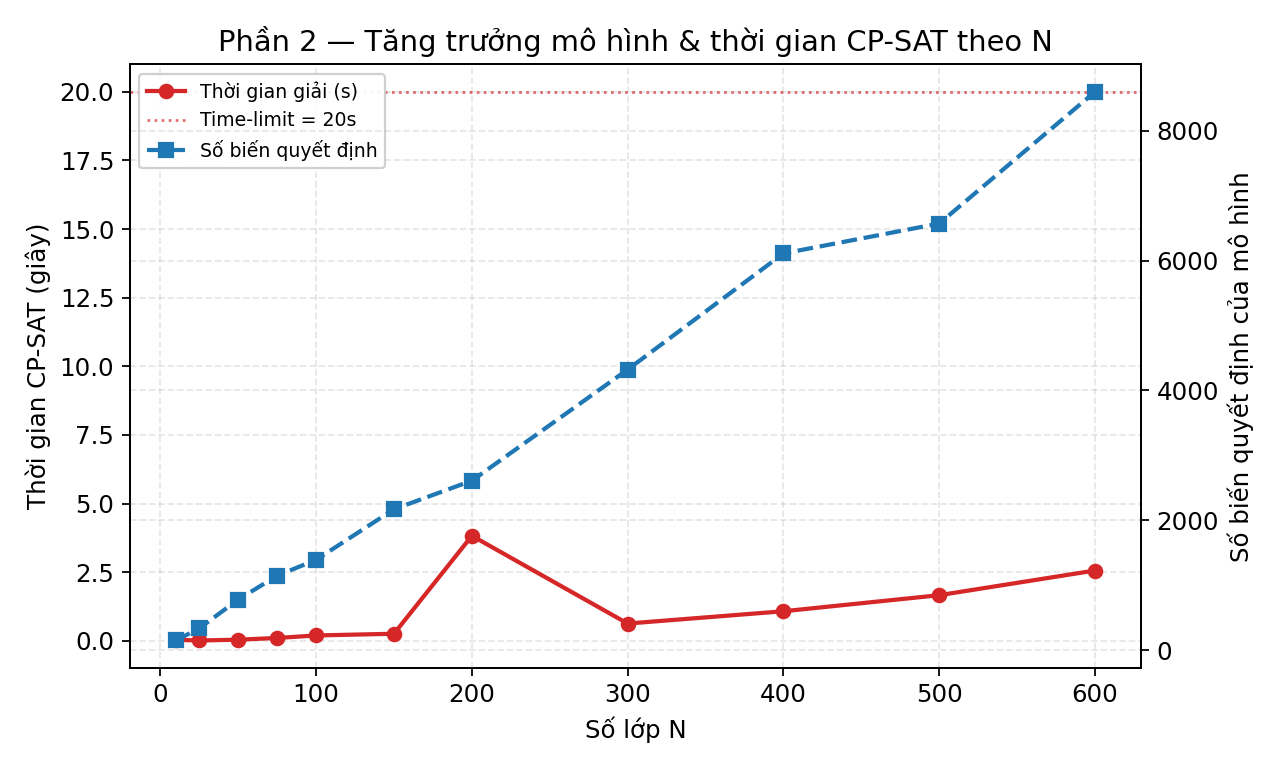
\includegraphics[width=0.74\textwidth]{figures/cpsat_scaling.png}
  \caption{Dữ liệu thưa: số biến (xanh) tăng tuyến tính theo $N$, nhưng thời gian
  giải (đỏ) vẫn xa dưới time-limit. Kích thước một mình không đánh gục CP-SAT.}
  \label{fig:cpsat}
\end{figure}

\begin{table}[ht]
\centering\small
\caption{CP-SAT trên dữ liệu ngẫu nhiên ``loose'' ($M=8$): số biến và thời gian
tăng theo $N$, vẫn chứng minh được tối ưu.}
\label{tab:cpsat-scaling}
\begin{tabular}{rrrlrr}
\toprule
$N$ & Số biến & Thời gian (s) & Trạng thái & $Q$ (obj) & Gap \\
\midrule
10 & 152 & 0.04 & OPTIMAL & 10 & 0 \\
25 & 339 & 0.01 & OPTIMAL & 25 & 0 \\
50 & 782 & 0.04 & OPTIMAL & 48 & 0 \\
75 & 1149 & 0.10 & OPTIMAL & 69 & 0 \\
100 & 1394 & 0.20 & OPTIMAL & 98 & 0 \\
150 & 2172 & 0.26 & OPTIMAL & 146 & 0 \\
200 & 2612 & 3.83 & OPTIMAL & 198 & 0 \\
300 & 4322 & 0.63 & OPTIMAL & 232 & 0 \\
400 & 6110 & 1.08 & OPTIMAL & 255 & 0 \\
500 & 6570 & 1.66 & OPTIMAL & 294 & 0 \\
600 & 8598 & 2.56 & OPTIMAL & 306 & 0 \\
\bottomrule
\end{tabular}
\end{table}

\begin{table}[ht]
\centering\small
\caption{CP-SAT trên dữ liệu thực nghẽn tài nguyên (time-limit $20$s). Khi $N$
lớn, solver chỉ đạt \textsc{feasible} với gap dương: không kịp chứng minh tối ưu.}
\label{tab:cpsat-real}
\begin{tabular}{lrrrrlrrrr}
\toprule
Instance & $N$ & $M$ & Số biến & Wall (s) & Trạng thái & Greedy & $Q$ & Cận trên & Gap \\
\midrule
\texttt{hustack01} & 200 & 10 & 3074 & 20.36 & FEASIBLE & 182 & 196 & 197 & 1 \\
\texttt{hustack02} & 500 & 50 & 38868 & 20.51 & FEASIBLE & 410 & 410 & 418 & 8 \\
\texttt{test08} & 1000 & 50 & 60002 & 20.93 & FEASIBLE & 959 & 961 & 1000 & 39 \\
\bottomrule
\end{tabular}
\end{table}


\noindent Kết quả Bảng~\ref{tab:cpsat-real} là minh chứng cho luận điểm trung tâm:
đối lập với dữ liệu thưa (tối ưu tới $N{=}600$), trên cả ba instance thực nghẽn tài
nguyên CP-SAT \emph{không đóng được khoảng cách} trong $20$s --- đều dừng ở
\textsc{feasible} với gap dương ngay cả khi đã warm-start (\texttt{hustack01}
$N{=}200$ gap $1$; \texttt{hustack02} $N{=}500$ gap $8$; \texttt{test08} $N{=}1000$
gap $39$). Đây là cơ sở định lượng cho ngưỡng $N\le 100$ của bộ định tuyến: vượt
ngưỡng, nguy cơ chỉ nhận nghiệm \textsc{feasible} là quá cao, buộc chuyển sang Local
Search (Mục~\ref{sec:ls}) và ALNS (Mục~\ref{sec:alns}).

% ===================== 5. LOCAL SEARCH — EJECTION CHAIN =====================
\section{Local Search (LS) với cơ chế Ejection Chain}
\label{sec:ls}

Tầng Heuristic phục vụ ngữ cảnh \emph{phản hồi nhanh}: cải thiện nghiệm Greedy
thường trong mili-giây (tới vài giây trên instance lớn nghẽn), đủ nhanh cho công
cụ chỉnh lịch tương tác và nhanh hơn ALNS nhiều bậc.

\subsection{Tư duy thuật toán: phá vỡ bế tắc của Greedy}
Greedy phụ thuộc thứ tự xử lý nên thường để sót những lớp bị \emph{một} lớp khác
chặn chỗ: lớp $u$ không còn vị trí nào trống chỉ vì lớp $v$ đang chiếm đúng khe nó
cần. Local Search nhắm chính vào thế bế tắc này: thay vì chấp nhận bỏ $u$, nó thử
\emph{tái sắp xếp} để giải phóng chỗ.

\subsection{Cơ chế chuỗi thay thế (Giải phóng -- Chèn -- Tái định vị)}
Mỗi vòng chọn ngẫu nhiên một lớp chờ $u$ và áp một toán tử lân cận duy nhất ---
\emph{Ejection Chain} (Thuật toán~\ref{alg:ls}): chèn trực tiếp nếu còn chỗ; nếu
không thì thực hiện ba bước:
\begin{itemize}
  \item \textbf{Giải phóng lớp $v$:} xóa bỏ lớp $v$ đang xếp khỏi vị trí hiện tại
  để giải phóng không gian thời gian/phòng học;
  \item \textbf{Chèn lớp $u$:} đặt lớp $u$ vào chỗ vừa trống (toán tử Insertion
  chuẩn);
  \item \textbf{Tái định vị lớp $v$:} tìm một tọa độ không gian--thời gian mới phù
  hợp cho lớp $v$ vừa bị đẩy ra.
\end{itemize}

\begin{figure}[H]
\centering
\begin{tikzpicture}[
  node distance=0.8cm and 1.5cm,
  >={Stealth[round]},
  class/.style={draw, thick, rounded corners=2pt, align=center, minimum height=0.7cm, minimum width=1.5cm},
  u/.style={class, fill=accent!15, draw=accent},
  v/.style={class, fill=cfast!15, draw=cfast},
  slot/.style={draw, dashed, thick, rounded corners=2pt, minimum height=0.7cm, minimum width=1.5cm, fill=black!5},
  lbl/.style={font=\scriptsize\itshape, align=center},
  arr/.style={->, thick, shorten >=2pt, shorten <=2pt}
]

  % Lớp U
  \node[u] (u) {Lớp chờ $u$};
  
  % Slot 1 (đang bị V chiếm)
  \node[slot, right=2cm of u] (s1) {};
  \node[v] (v) at (s1) {Lớp $v$};
  \node[lbl, above=0.1cm of s1] {Chỗ duy nhất cho $u$\\ (đang bị chiếm)};

  % Slot 2 (trống)
  \node[slot, right=2cm of s1] (s2) {Trống};
  \node[lbl, above=0.1cm of s2] {Chỗ mới cho $v$};

  % Các mũi tên
  \draw[arr, accent, out=20, in=160] (u) to node[lbl, above] {1. Chèn $u$} (s1);
  \draw[arr, cscale, out=-20, in=200] (v.south) to node[lbl, below] {2. Giải phóng $v$} (s2.south west);
  \draw[arr, cfast, out=20, in=160] (v.north) to node[lbl, above] {3. Tái định vị $v$} (s2.north west);

\end{tikzpicture}
\caption{Cơ chế Ejection Chain: Lớp $u$ cần chỗ, hệ thống \emph{giải phóng} lớp $v$ đang chiếm chỗ đó, rồi \emph{tái định vị} $v$ vào một chỗ trống khác.}
\label{fig:ejection-chain}
\end{figure}

\begin{algorithm}[H]
\caption{Local Search bằng Ejection Chain}
\label{alg:ls}
\KwIn{nghiệm Greedy; tập lớp chưa xếp $U$}
\For{mỗi bước lặp \textbf{và} $U\neq\varnothing$ \textbf{và} chưa hết ngân sách}{
  chọn ngẫu nhiên lớp chờ $u\in U$\;
  \uIf{chèn trực tiếp $u$ được}{chèn $u$; cập nhật nghiệm tốt nhất\;}
  \Else{
    giải phóng một lớp $v$ đang xếp; chèn $u$ vào chỗ vừa trống\;
    \uIf{tìm được chỗ mới cho $v$}{tái định vị $v$ (số lớp không đổi, cấu trúc mới)\;}
    \uElseIf{$t_u < t_v$}{giữ $u$ (tốn ít tiết hơn $\Rightarrow$ lợi về sau)\;}
    \Else{hoàn tác: trả $v$ về chỗ cũ\;}
  }
}
\Return nghiệm tốt nhất đã lưu\;
\end{algorithm}

\subsection{Đánh giá chênh lệch và điều kiện chấp nhận (First Improvement)}
LS theo chiến lược \emph{First Improvement}: chấp nhận ngay nước đi đầu tiên
\emph{có lợi} thay vì duyệt toàn bộ lân cận tìm nước tốt nhất --- ưu tiên tốc độ.
Tiêu chí ``có lợi'' rất gọn: nếu tái định vị được $v$ thì giữ (Q không giảm, cấu
trúc đổi, mở cơ hội mới); nếu không thì chỉ giữ $u$ khi $t_u<t_v$ (đổi một lớp dài
lấy một lớp ngắn, giải phóng tài nguyên ròng), ngược lại hoàn tác. Nhờ luôn lưu
\emph{nghiệm tốt nhất} qua \texttt{snapshot}, số lớp xếp được \emph{không bao giờ
giảm}.

\subsection{Giới hạn của thuật toán (Hiệu ứng Plateau)}
Ejection Chain chỉ thay đổi \emph{cục bộ} (đổi chỗ từng cặp lớp). Khi mọi hoán đổi
đơn lẻ đều không mở thêm chỗ, lời giải mắc kẹt trên một \emph{cao nguyên}: nó không
thể tạo biến đổi vĩ mô (ví dụ tái tổ chức toàn bộ lịch của một giáo viên quá tải).
Đây không phải lỗi cài đặt mà là \emph{giới hạn bản chất} của tìm kiếm cục bộ với
một toán tử --- và là động lực trực tiếp cho ALNS ở Mục~\ref{sec:alns}, nơi cơ chế
phá hủy quy mô lớn cho phép nhảy ra khỏi cao nguyên.

% ===================== 6. ALNS =====================
\section{Thuật toán Adaptive Large Neighborhood Search (ALNS)}
\label{sec:alns}

Tầng Metaheuristic phục vụ ngữ cảnh \emph{quy mô lớn, chạy theo lô}, nơi cần chất
lượng cao và sẵn sàng đổi vài giây tính toán. ALNS hoạt động theo chu trình
\emph{phá hủy \& tái tạo} (ruin \& recreate): mỗi vòng phá $\sim 15\%$ số lớp đang
xếp rồi tái tạo bằng một cặp toán tử được chọn thích nghi, sau đó quyết định chấp
nhận theo Simulated Annealing. Tổng quan ở Thuật toán~\ref{alg:alns}.

\subsection{Ba toán tử Phá hủy (Random, Worst-Time, Related-Teacher)}
Mỗi toán tử nhắm một dạng bế tắc khác nhau:
\begin{itemize}
  \item \opt{Random}: gỡ ngẫu nhiên $k$ lớp --- đa dạng hóa, tránh thiên kiến.
  \item \opt{Worst-Time}: gỡ $k$ lớp \emph{thời lượng lớn nhất} --- giải phóng các
  khối thời gian cồng kềnh, chiếm nhiều tài nguyên nhất.
  \item \opt{Related-Teacher}: chọn giáo viên có lịch dày nhất rồi gỡ cụm lớp của
  họ --- tập trung tháo gỡ điểm xung đột.
\end{itemize}

Hình~\ref{fig:destroy-ops} minh họa ba toán tử trên cùng một lịch hiện tại (khối
$=$ lớp đang xếp; khối tô đỏ nét đứt $=$ lớp bị gỡ).

\begin{figure}[H]
\centering
\begin{tikzpicture}[
  font=\scriptsize,
  blk/.style={draw, thick, minimum height=0.55cm, fill=black!8, inner sep=1pt},
  rem/.style={blk, fill=cscale!22, draw=cscale, dashed, very thick, text=cscale},
  t1/.style={blk, fill=cfast!18, draw=cfast!70},
  t2/.style={blk, fill=cexact!16, draw=cexact!70},
  t1r/.style={blk, fill=cfast!18, draw=cscale, dashed, very thick, text=cscale},
  opcap/.style={font=\scriptsize\bfseries, align=center},
]
% ---------- (a) Random ----------
\begin{scope}
  \node[blk,minimum width=0.7cm] (a1) at (0,0){A};
  \node[rem,minimum width=0.7cm, right=2pt of a1] (a2){B\,$\times$};
  \node[blk,minimum width=0.7cm, right=2pt of a2] (a3){C};
  \node[rem,minimum width=0.7cm, right=2pt of a3] (a4){D\,$\times$};
  \node[blk,minimum width=0.7cm, right=2pt of a4] (a5){E};
  \node[opcap] at (1.9,-0.75) {(a) \opt{Random}};
  \node[font=\scriptsize] at (1.9,-1.15) {gỡ $k$ lớp bất kỳ};
\end{scope}
% ---------- (b) Worst-Time ----------
\begin{scope}[xshift=5.5cm]
  \node[blk,minimum width=0.5cm] (b1) at (0,0){};
  \node[blk,minimum width=1.0cm, right=2pt of b1] (b2){};
  \node[blk,minimum width=0.5cm, right=2pt of b2] (b3){};
  \node[rem,minimum width=1.6cm, right=2pt of b3] (b4){dài\,$\times$};
  \node[opcap] at (1.9,-0.75) {(b) \opt{Worst-Time}};
  \node[font=\scriptsize] at (1.9,-1.15) {gỡ lớp thời lượng lớn nhất};
\end{scope}
% ---------- (c) Related-Teacher ----------
\begin{scope}[xshift=11cm]
  \node[t1r,minimum width=0.7cm] (c1) at (0,0){$g_1$};
  \node[t2,minimum width=0.7cm, right=2pt of c1] (c2){$g_2$};
  \node[t1r,minimum width=0.7cm, right=2pt of c2] (c3){$g_1$};
  \node[t2,minimum width=0.7cm, right=2pt of c3] (c4){$g_2$};
  \node[t1r,minimum width=0.7cm, right=2pt of c4] (c5){$g_1$};
  \node[opcap] at (1.9,-0.75) {(c) \opt{Related-Teacher}};
  \node[font=\scriptsize] at (1.9,-1.15) {gỡ cụm lớp của 1 giáo viên};
\end{scope}
\end{tikzpicture}
\caption{Ba toán tử Phá hủy. \opt{Random} gỡ ngẫu nhiên; \opt{Worst-Time} gỡ khối
thời lượng dài nhất; \opt{Related-Teacher} gỡ toàn bộ lớp của giáo viên dày lịch
nhất ($g_1$).}
\label{fig:destroy-ops}
\end{figure}

\subsection{Ba toán tử Sửa chữa (Greedy, Regret-2, First-Possible)}
\begin{itemize}
  \item \opt{Greedy}: chèn lại theo sĩ số rồi thời lượng giảm dần, mỗi lớp vào vị
  trí trống đầu tiên.
  \item \opt{Regret-2}: ưu tiên lớp ``hối tiếc'' cao --- lớp càng ít phòng khả thi
  (đếm bằng \texttt{feasible\_room\_count}) thì điểm $1/\text{cnt}$ càng lớn, được
  chèn trước để không bị kẹt về sau.
  \item \opt{First-Possible}: xáo trộn ngẫu nhiên rồi chèn vào chỗ đầu tiên --- tạo
  nhiễu cấu trúc.
\end{itemize}

Ba toán tử khác nhau ở \emph{thứ tự ưu tiên} các lớp chờ khi chèn lại
(Hình~\ref{fig:repair-ops}); số trong vòng tròn là thứ tự chèn.

\begin{figure}[H]
\centering
\begin{tikzpicture}[
  font=\scriptsize,
  blk/.style={draw, thick, minimum height=0.6cm, fill=black!8, inner sep=2pt},
  hl/.style={blk, fill=accent!20, draw=accent, very thick},
  ord/.style={circle, draw=accent, fill=accent!85, text=white, font=\tiny,
              inner sep=0.6pt, minimum size=0.34cm},
  opcap/.style={font=\scriptsize\bfseries, align=center},
  sub/.style={font=\scriptsize, align=center},
]
% ---------- (a) Greedy ----------
\begin{scope}
  \node[blk,minimum width=1.0cm] (g1) at (0,0){$s{=}80$};
  \node[blk,minimum width=1.0cm, right=4pt of g1] (g2){$s{=}50$};
  \node[blk,minimum width=1.0cm, right=4pt of g2] (g3){$s{=}20$};
  \node[ord, above=1pt of g1]{1}; \node[ord, above=1pt of g2]{2}; \node[ord, above=1pt of g3]{3};
  \node[opcap] at (1.6,-0.7) {(a) \opt{Greedy}};
  \node[sub] at (1.6,-1.1) {sĩ số giảm dần};
\end{scope}
% ---------- (b) Regret-2 ----------
\begin{scope}[xshift=5.3cm]
  \node[hl,minimum width=1.7cm] (rB) at (0,0){$u_B$: 1 phòng};
  \node[blk,minimum width=1.7cm, right=4pt of rB] (rA){$u_A$: 3 phòng};
  \node[ord, above=1pt of rB]{1}; \node[ord, above=1pt of rA]{2};
  \node[opcap] at (1.95,-0.7) {(b) \opt{Regret-2}};
  \node[sub] at (1.95,-1.1) {ít phòng khả thi $\to$ chèn trước};
\end{scope}
% ---------- (c) First-Possible ----------
\begin{scope}[xshift=11.3cm]
  \node[blk,minimum width=0.8cm] (f1) at (0,0){$u_1$};
  \node[blk,minimum width=0.8cm, right=4pt of f1] (f2){$u_2$};
  \node[blk,minimum width=0.8cm, right=4pt of f2] (f3){$u_3$};
  \node[ord, above=1pt of f1]{2}; \node[ord, above=1pt of f2]{1}; \node[ord, above=1pt of f3]{3};
  \node[opcap] at (1.45,-0.7) {(c) \opt{First-Possible}};
  \node[sub] at (1.45,-1.1) {thứ tự ngẫu nhiên};
\end{scope}
\end{tikzpicture}
\caption{Ba toán tử Sửa chữa khác nhau ở thứ tự chọn lớp chờ để chèn (số trong
vòng tròn). \opt{Greedy} theo sĩ số giảm dần; \opt{Regret-2} ưu tiên lớp ít phòng
khả thi nhất ($u_B$); \opt{First-Possible} theo thứ tự xáo trộn ngẫu nhiên. Cả ba
đều đặt mỗi lớp vào vị trí trống đầu tiên tìm được.}
\label{fig:repair-ops}
\end{figure}

\subsection{Cập nhật trọng số Adaptive Roulette-Wheel ($\pi_1,\pi_2,\pi_3$)}
Mỗi toán tử mang trọng số $w_j$ (khởi tạo $1$); toán tử được bốc bằng bánh xe
roulette với xác suất tỉ lệ trọng số:
\begin{equation}
  p_j = \frac{w_j}{\sum_\ell w_\ell}.
  \label{eq:roulette}
\end{equation}
Sau mỗi vòng, toán tử vừa dùng nhận điểm thưởng $\pi$ theo mức đóng góp --- tạo
nghiệm tốt nhất mới ($\pi_1{=}10$), cải thiện nghiệm hiện hành ($\pi_2{=}5$), được
SA chấp nhận dù không cải thiện ($\pi_3{=}2$), bị bác ($0$) --- rồi trọng số cập
nhật theo trung bình trượt mũ với hệ số học $\lambda$:
\begin{equation}
  w_j \leftarrow \lambda\,w_j + (1-\lambda)\,\pi.
  \label{eq:update}
\end{equation}

\subsection{Tiêu chí chấp nhận bằng Luyện kim mô phỏng (Simulated Annealing)}
Để thoát cực trị cục bộ, nghiệm lùi bước vẫn được chấp nhận với xác suất Boltzmann
$\exp(-\Delta/T)$, với $\Delta=Q_\text{best}-Q_\text{new}\ge 0$ và nhiệt độ giảm
dần $T\leftarrow\alpha T$ ($T_0{=}10,\ \alpha{=}0.98$). Đầu chạy ($T$ lớn) ưu tiên
khám phá; cuối chạy ($T\to 0$) ưu tiên khai thác.

\begin{figure}[H]
\centering
\begin{tikzpicture}[
  >={Stealth[round]},
  box/.style={draw, thick, rounded corners=3pt, align=center, minimum height=0.9cm, font=\small},
  state/.style={box, fill=black!5, minimum width=2.0cm},
  op/.style={box, fill=accent!10, draw=accent, minimum width=2.4cm},
  dec/.style={box, diamond, aspect=2, fill=cscale!10, draw=cscale, inner sep=1pt, font=\scriptsize\bfseries, align=center},
  lbl/.style={font=\scriptsize, align=center},
  arr/.style={->, thick}
]
  \node[state] (s1) {Nghiệm hiện tại\\$s_\text{cur}$};
  \node[op, right=1.1cm of s1] (ruin) {Phá hủy (Ruin)\\ \scriptsize gỡ $\sim 15\%$ lớp};
  \node[op, right=0.9cm of ruin] (rec) {Sửa chữa (Recreate)\\ \scriptsize chèn lại cấu trúc};
  \node[state, right=1.1cm of rec] (s2) {Ứng viên\\$s_\text{new}$};
  \node[dec, below=1.25cm of s2] (sa) {SA\\Accept?};
  \node[op, below=1.25cm of s1] (update) {Cập nhật trọng số\\ \scriptsize (Roulette, $\pi$)};

  \draw[arr] (s1) -- (ruin);
  \draw[arr] (ruin) -- node[lbl, above] {lớp bị gỡ} (rec);
  \draw[arr] (rec) -- (s2);
  \draw[arr] (s2) -- (sa);
  \draw[arr] (sa) -- node[lbl, above, align=center]
        {\textbf{Có:} nhận $s_\text{new}$\\\textbf{Không:} khôi phục $s_\text{best}$} (update);
  \draw[arr] (update) -- node[lbl, left] {vòng lặp\\tiếp theo} (s1);
\end{tikzpicture}
\caption{Chu trình Phá hủy \& Sửa chữa (Ruin \& Recreate) của ALNS kết hợp đánh giá chấp nhận bằng Luyện kim mô phỏng (SA) và cập nhật trọng số toán tử (Adaptive).}
\label{fig:alns-loop}
\end{figure}

\begin{algorithm}[H]
\caption{ALNS = Ruin \& Recreate $+$ Adaptive $+$ Simulated Annealing}
\label{alg:alns}
\KwIn{hạt giống Greedy; $T_0,\alpha,\lambda,(\pi_1,\pi_2,\pi_3)$}
$s_\text{best}\leftarrow s_\text{cur}\leftarrow$ Greedy; $T\leftarrow T_0$\;
\For{mỗi vòng lặp (tới khi hết ngân sách hoặc xếp đủ $N$ lớp)}{
  bốc cặp (Phá hủy, Sửa chữa) theo roulette~\eqref{eq:roulette}\;
  phá $\lceil 0.15\,Q\rceil$ lớp; tái tạo $\Rightarrow s_\text{new}$\;
  \uIf{$Q_\text{new}>Q_\text{best}$}{nhận; $s_\text{best}\leftarrow s_\text{new}$; $\pi\leftarrow\pi_1$\;}
  \uElseIf{$Q_\text{new}>Q_\text{cur}$}{nhận; $\pi\leftarrow\pi_2$\;}
  \uElseIf{$\text{rand}()<e^{-\Delta/T}$}{nhận (lùi bước); $\pi\leftarrow\pi_3$\;}
  \Else{khôi phục $s_\text{best}$; $\pi\leftarrow 0$\;}
  cập nhật trọng số~\eqref{eq:update}; \quad $T\leftarrow\alpha T$\;
}
\Return $s_\text{best}$\;
\end{algorithm}

% ===================== 7. PARAMETER TUNING =====================
\section{Phân tích độ nhạy và tinh chỉnh tham số (Parameter Tuning)}
\label{sec:tuning}

Mỗi tham số của ALNS được biện minh bằng đồ thị độ nhạy, không phải chọn tùy ý.
Mọi thí nghiệm chạy trên instance nghẽn \texttt{test09} ($N{=}200$, $M{=}5$) ---
nơi động lực học bộc lộ rõ nhất --- lấy trung bình $5$ hạt giống ngẫu nhiên.

\subsection{Sự tiến hóa của xác suất chọn toán tử (cân bằng Khám phá -- Khai thác)}
\begin{figure}[H]
  \centering
  \begin{subfigure}{0.49\textwidth}
    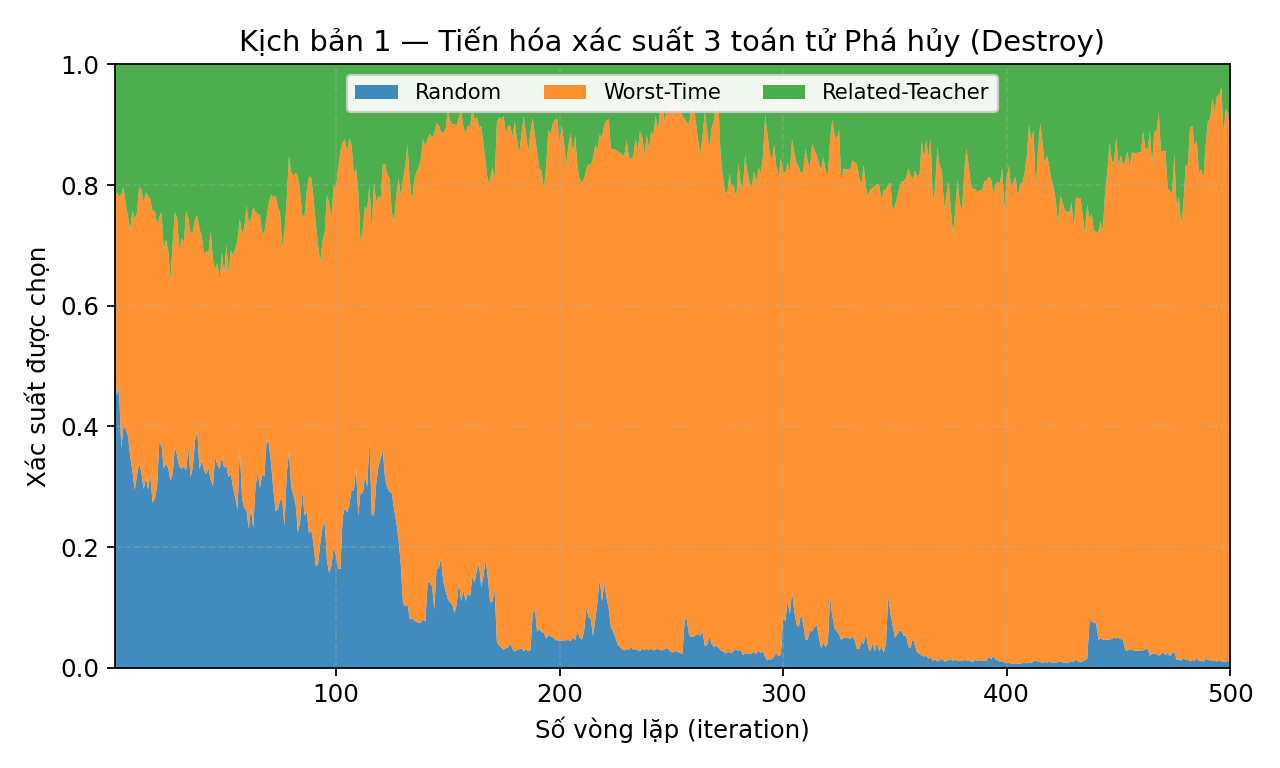
\includegraphics[width=\linewidth]{figures/s1_destroy_probability.png}
    \caption{Toán tử Phá hủy}
  \end{subfigure}\hfill
  \begin{subfigure}{0.49\textwidth}
    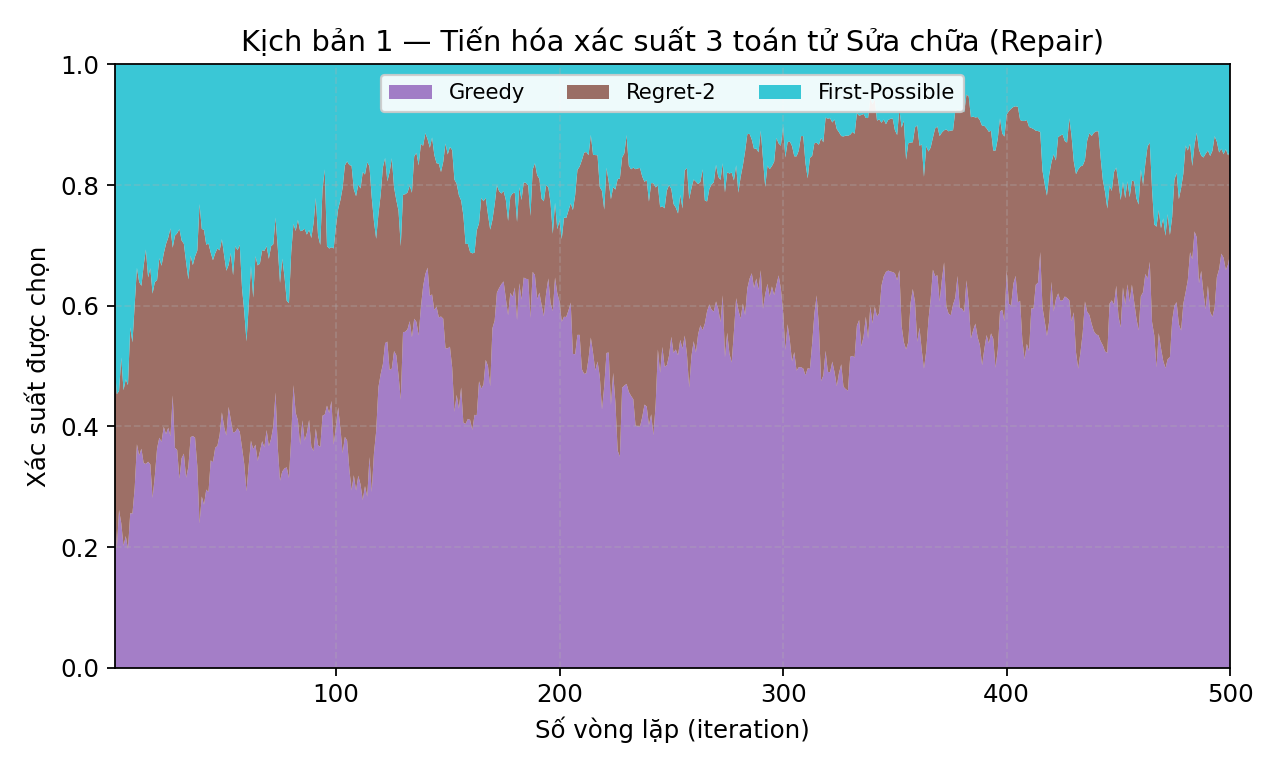
\includegraphics[width=\linewidth]{figures/s1_repair_probability.png}
    \caption{Toán tử Sửa chữa}
  \end{subfigure}
  \caption{Miền xác suất chọn toán tử theo vòng lặp (tổng mỗi cột $=1$), tính
  theo~\eqref{eq:roulette}.}
  \label{fig:s1}
\end{figure}

\noindent Hình~\ref{fig:s1} cho thấy cơ chế thích nghi \emph{thực sự học}: khởi đầu
gần đồng đều (giai đoạn \emph{khám phá}), thuật toán nhanh chóng dồn xác suất cho
\opt{Worst-Time} (tỉ trọng cuối $\approx 0.89$) và \opt{Greedy} bên sửa chữa
($\approx 0.69$) --- giai đoạn \emph{khai thác} chiến lược hiệu quả nhất trên
instance nghẽn phòng, trong khi phá ngẫu nhiên bị đào thải. Đây là minh chứng định
lượng cho giá trị của adaptive selection.

\subsection{Tác động của hệ số học $\lambda$ (Learning Rate)}
\begin{figure}[H]
  \centering
  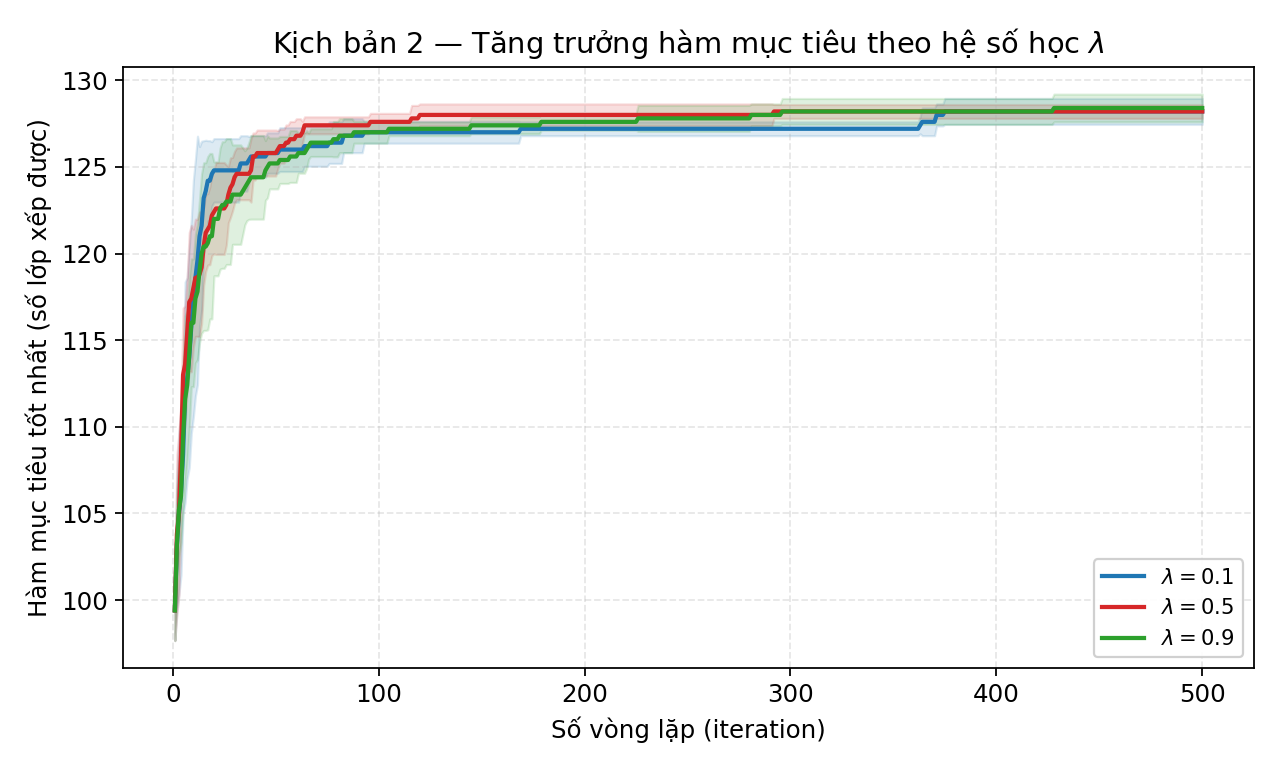
\includegraphics[width=0.70\textwidth]{figures/s2_lambda_convergence.png}
  \caption{Tăng trưởng hàm mục tiêu theo $\lambda\in\{0.1,0.5,0.9\}$; dải mờ là
  $\pm 1$ độ lệch chuẩn trên $5$ hạt giống.}
  \label{fig:s2}
\end{figure}

\noindent Ba giá trị cho chất lượng trung bình gần như nhau ($\approx 128$ lớp),
nên tiêu chí phân định là \emph{độ ổn định}: $\lambda{=}0.5$ cho độ lệch chuẩn cuối
kỳ ($\sigma\approx 0.40$) nhỏ hơn $\sim 2\times$ so với $\lambda{=}0.1$ (quên nhanh,
$\sigma\approx 0.75$) và $\lambda{=}0.9$ (ì, $\sigma\approx 0.80$). Ta chọn
$\boxed{\lambda=0.5}$ vì hành vi tái lập và đáng tin cậy nhất.

\subsection{Sự biến thiên Nhiệt độ $T$ và hệ số làm mát $\alpha$ (Cooling Schedule)}
\begin{figure}[H]
  \centering
  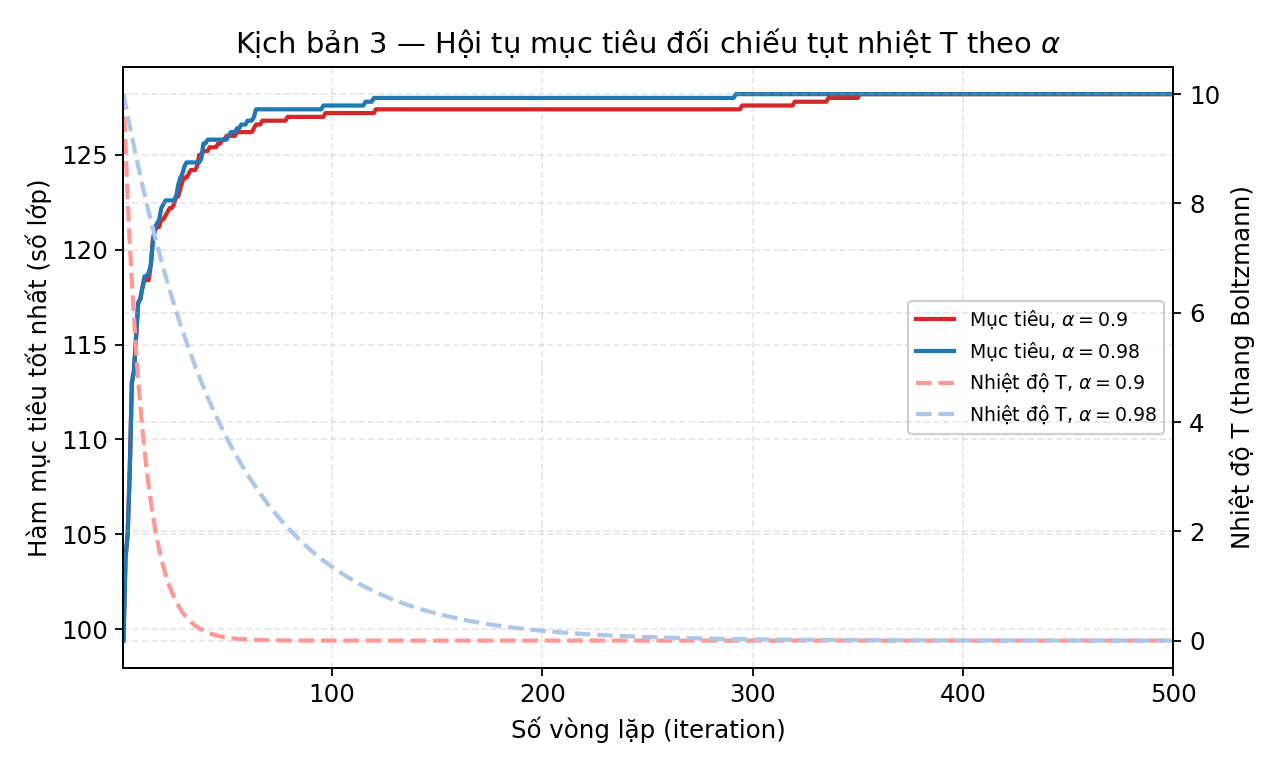
\includegraphics[width=0.76\textwidth]{figures/s3_temperature_dualaxis.png}
  \caption{Đồ thị kép: hội tụ mục tiêu (đường liền, trục trái) đối chiếu tụt nhiệt
  $T$ (đường đứt, trục phải) cho $\alpha=0.90$ và $\alpha=0.98$.}
  \label{fig:s3}
\end{figure}

\noindent Với $\alpha{=}0.90$, nhiệt độ rơi về $\approx 0.06$ chỉ sau $\sim 50$
vòng --- sau đó $e^{-\Delta/T}\approx 0$, thuật toán \emph{đóng băng} thành leo đồi
thuần túy, dễ chết yểu ở cực trị cục bộ. Với $\alpha{=}0.98$, $T$ còn $\approx 3.7$
tại vòng $50$ và chỉ tiệm cận $0$ quanh vòng $250$, giữ ``van xả'' khám phá lâu hơn
mà gần như không tốn thêm chi phí. Ta chọn $\boxed{T_0=10,\ \alpha=0.98}$.

% ===================== 8. KẾT QUẢ THỰC NGHIỆM =====================
\section{Kết quả thực nghiệm}
\label{sec:results}

\subsection{Thiết lập đánh giá công bằng (Môi trường, Time-limit, Seeds)}
\label{sec:setup}
Để so sánh công bằng, mọi thuật toán được đặt trên cùng một sân chơi:
\begin{itemize}
  \item \textbf{Ngân sách thời gian chung:} mỗi instance, LS, ALNS và CP-SAT cùng
  nhận \emph{một} time-limit $30$s. Giá trị này xuất phát từ chi phí thực đo của
  ALNS (toán tử Regret-2 $\approx 0.5$s/vòng trên $N{=}500$, cần $\sim 50$--$100$
  vòng để phát huy); $30$s cũng phù hợp ngữ cảnh xếp lịch theo lô. Để không lãng
  phí ngân sách trên instance dễ, ALNS \emph{dừng sớm} khi đã xếp đủ $N$ lớp. Ngân
  sách là ``mềm'' (kiểm tra giữa các vòng): một vòng Regret-2 trên $N$ lớn có thể
  kéo dài vài giây nên ALNS đôi khi vượt nhẹ $30$s (tới $\sim 37$s) --- điều này chỉ
  \emph{có lợi} cho ALNS, vậy mà nó vẫn thua LS trên instance lớn nghẽn.
  \item \textbf{Seed cố định:} các thuật toán ngẫu nhiên (LS, ALNS) lặp với bộ seed
  cố định lấy từ $\{1,7,13,21,42\}$ --- $3$ lần (nhóm nhỏ/vừa) và $2$ lần (nhóm lớn,
  do chi phí cao) --- báo cáo $(\min,\max,\text{avg},\text{std})$ để tái lập.
  \item \textbf{Cô lập:} mỗi lần chạy nạp lại instance sạch; Greedy là hạt giống
  chung. Ngoài ra ta ghi thêm cột \emph{LS (hội tụ)} --- LS dừng tự nhiên --- để
  phản ánh đặc tính phản hồi nhanh của tầng Heuristic.
\end{itemize}

\begin{table}[H]
\centering\small
\caption{Môi trường thực nghiệm và giao thức đánh giá công bằng.}
\label{tab:bench-env}
\begin{tabular}{ll}
\toprule
Hạng mục & Giá trị \\
\midrule
Hệ điều hành & \texttt{macOS-26.3.1-arm64-arm-64bit} \\
CPU & \texttt{arm} (11 nhân) \\
Python & 3.10.20 \\
OR-Tools & 9.15.6755 \\
Ngân sách thời gian chung & 30 giây / instance (LS, ALNS, CP-SAT) \\
Số lần lặp (seed) & 3 (nhỏ/vừa), 2 (lớn) \\
Tập seed & lấy từ \{1, 7, 13, 21, 42\} \\
\bottomrule
\end{tabular}
\end{table}


\subsection{Bảng kết quả đầy đủ (phân nhóm: Nhỏ, Trung bình, Lớn)}
\label{sec:tables}
Ba nhóm dữ liệu bao phủ phổ quy mô và độ khó. Nhóm nhỏ có chuẩn CP-SAT tối ưu
(Bảng~\ref{tab:bench-small}); nhóm trung bình và lớn trộn instance dư tài nguyên
với instance nghẽn (Bảng~\ref{tab:bench-medium},~\ref{tab:bench-large}).

\begin{table}[H]
\centering\small
\caption{Nhóm nhỏ ($N\le 30$): CP-SAT là chuẩn tối ưu. LS/ALNS trung bình các seed.}
\label{tab:bench-small}
\begin{tabular}{lrr rr rr rr}
\toprule
Instance & $N$ & $M$ & CP-SAT & Greedy & LS avg & ALNS avg & \%opt(LS) & \%opt(ALNS) \\
\midrule
\texttt{test01} & 5 & 3 & 5 & 5 & 5.0 & 5.0 & 100\% & 100\% \\
\texttt{test03} & 20 & 5 & 20 & 20 & 20.0 & 20.0 & 100\% & 100\% \\
\texttt{hustack05} & 20 & 3 & 20 & 20 & 20.0 & 20.0 & 100\% & 100\% \\
\texttt{test02} & 10 & 5 & 10 & 10 & 10.0 & 10.0 & 100\% & 100\% \\
\texttt{hustack08} & 10 & 2 & 9 & 9 & 9.0 & 9.0 & 100\% & 100\% \\
\bottomrule
\end{tabular}
\end{table}

\begin{table}[H]
\centering\small
\caption{Nhóm trung bình ($N\approx 100$--$200$): trộn instance dư tài nguyên và nghẽn phòng ($M$ nhỏ). Cùng ngân sách $30$s.}
\label{tab:bench-medium}
\begin{tabular}{lrr r l ll l r}
\toprule
\multirow{2}{*}{Instance} & \multirow{2}{*}{$N$} & \multirow{2}{*}{$M$}
& \multirow{2}{*}{Greedy}
& \multicolumn{1}{c}{LS} & \multicolumn{2}{c}{ALNS} & \multirow{2}{*}{CP-SAT}
& \multirow{2}{*}{$\Delta$(ALNS$-$Gr)} \\
\cmidrule(lr){5-5}\cmidrule(lr){6-7}
& & & & min/avg/max & min/avg/max & std & & \\
\midrule
\texttt{test05} & 100 & 15 & 100 & 100/100.0/100 & 100/100.0/100 & 0.00 & 100 (OPTI) & +0.0 \\
\texttt{comp11} & 162 & 5 & 147 & 162/162.0/162 & 162/162.0/162 & 0.00 & 162 (OPTI) & +15.0 \\
\texttt{test09} & 200 & 5 & 125 & 127/127.0/127 & 127/128.3/129 & 0.94 & 131 (OPTI) & +3.3 \\
\texttt{hustack01} & 200 & 10 & 182 & 184/184.3/185 & 193/193.7/194 & 0.47 & 196 (FEAS) & +11.7 \\
\bottomrule
\end{tabular}
\end{table}

\begin{table}[H]
\centering\small
\caption{Nhóm lớn ($N\ge 500$). Cùng ngân sách $30$s; LS/ALNS trung bình các seed.}
\label{tab:bench-large}
\begin{tabular}{lrr r l ll l r}
\toprule
\multirow{2}{*}{Instance} & \multirow{2}{*}{$N$} & \multirow{2}{*}{$M$}
& \multirow{2}{*}{Greedy}
& \multicolumn{1}{c}{LS} & \multicolumn{2}{c}{ALNS} & \multirow{2}{*}{CP-SAT}
& \multirow{2}{*}{$\Delta$(ALNS$-$Gr)} \\
\cmidrule(lr){5-5}\cmidrule(lr){6-7}
& & & & min/avg/max & min/avg/max & std & & \\
\midrule
\texttt{test07} & 500 & 30 & 499 & 500/500.0/500 & 500/500.0/500 & 0.00 & 500 (OPTI) & +1.0 \\
\texttt{hustack02} & 500 & 50 & 410 & 415/415.5/416 & 410/410.5/411 & 0.50 & 410 (FEAS) & +0.5 \\
\texttt{hustack03} & 700 & 50 & 453 & 455/455.5/456 & 453/453.0/453 & 0.00 & 453 (FEAS) & +0.0 \\
\texttt{hustack09} & 800 & 50 & 477 & 478/478.0/478 & 477/477.0/477 & 0.00 & 478 (FEAS) & +0.0 \\
\texttt{test08} & 1000 & 50 & 959 & 982/982.5/983 & 1000/1000.0/1000 & 0.00 & 990 (FEAS) & +41.0 \\
\texttt{hustack10} & 1000 & 50 & 508 & 508/508.0/508 & 508/508.0/508 & 0.00 & 508 (OPTI) & +0.0 \\
\bottomrule
\end{tabular}
\end{table}


\subsection{Biểu đồ so sánh (chất lượng nghiệm và thời gian chạy)}
\label{sec:charts}
\begin{figure}[H]
  \centering
  \begin{subfigure}{0.49\textwidth}
    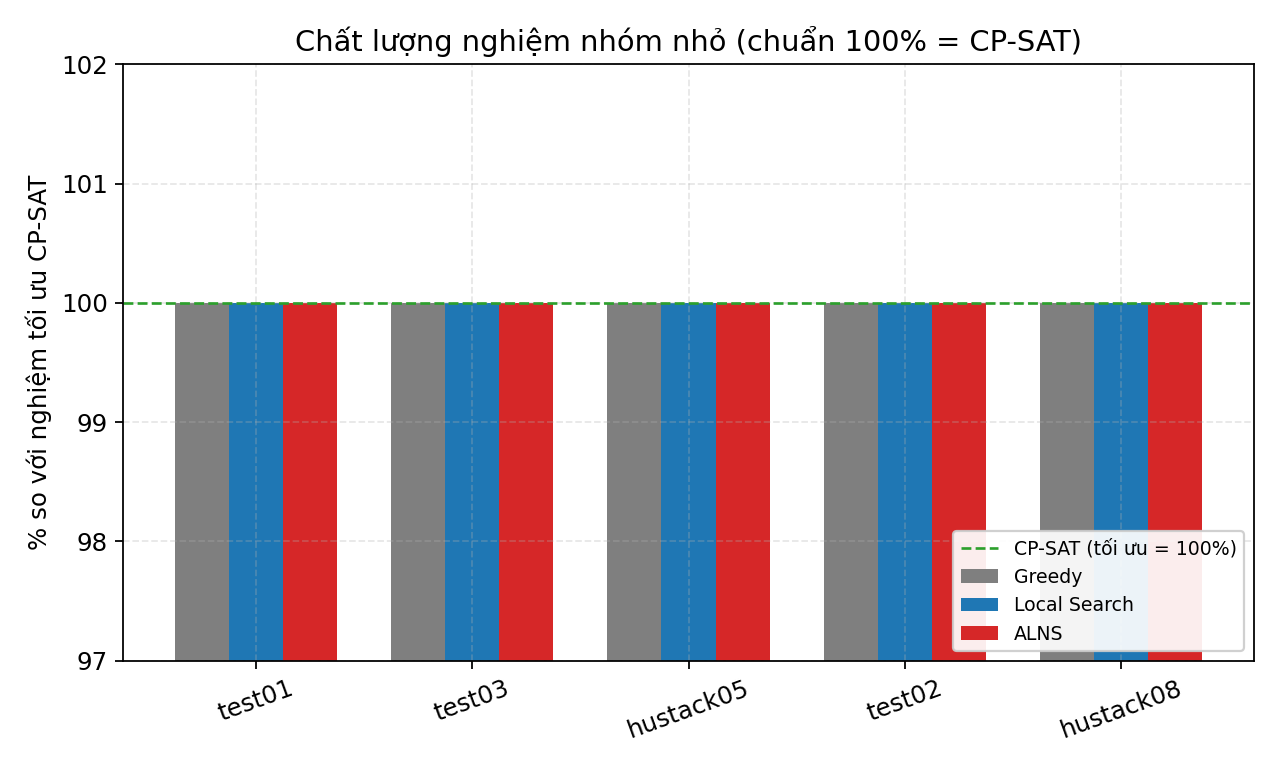
\includegraphics[width=\linewidth]{figures/bench_small_quality.png}
    \caption{Nhóm nhỏ: \% so với CP-SAT}
  \end{subfigure}\hfill
  \begin{subfigure}{0.49\textwidth}
    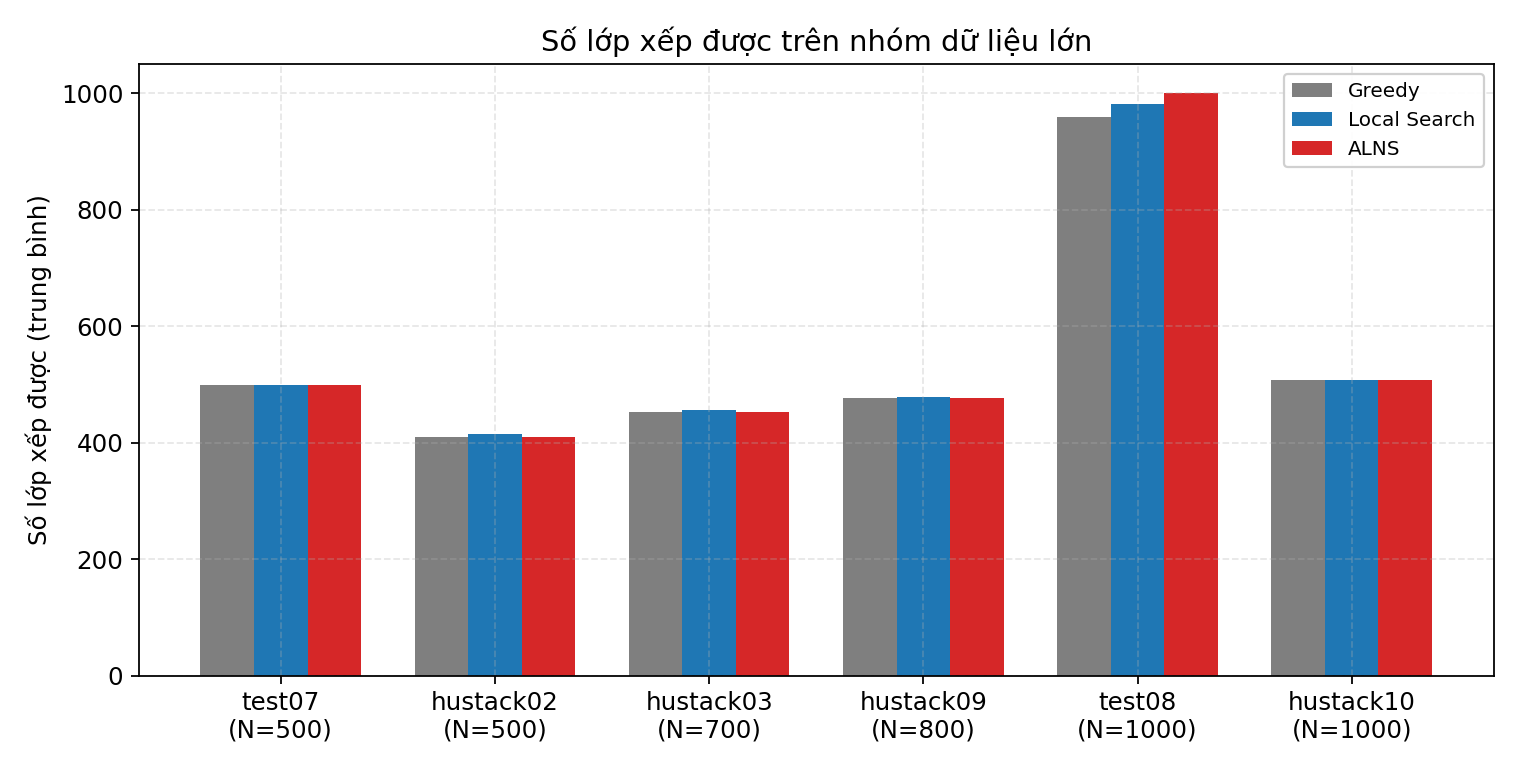
\includegraphics[width=\linewidth]{figures/bench_large_gain.png}
    \caption{Nhóm lớn: số lớp xếp được}
  \end{subfigure}
  \caption{Chất lượng nghiệm: nhóm nhỏ bám chuẩn tối ưu; nhóm lớn --- ALNS đạt tối
  ưu trên \texttt{test08} (còn khe cấu trúc lớn), còn trên các instance nghẽn HUStack
  thì LS nhỉnh hơn.}
  \label{fig:bench-quality}
\end{figure}

\begin{figure}[H]
  \centering
  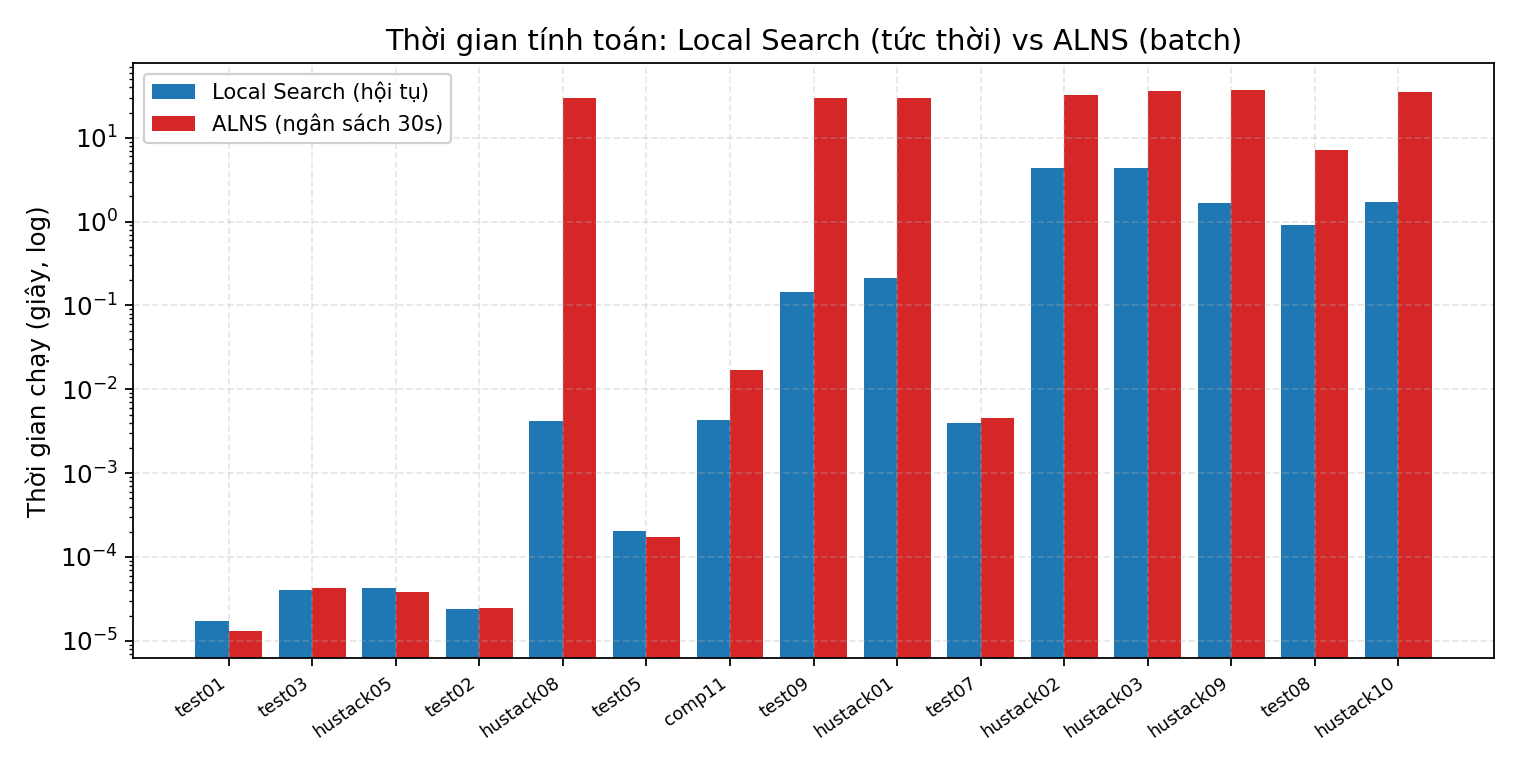
\includegraphics[width=0.82\textwidth]{figures/bench_runtime.png}
  \caption{Thời gian tính toán (thang log): Local Search hội tụ rất nhanh ---
  mili-giây trên dữ liệu nhỏ/thưa, tới vài giây trên instance lớn nghẽn (vd
  \texttt{hustack02} $\approx 4.4$s) --- vẫn nhanh hơn ALNS nhiều bậc; ALNS dùng
  trọn ngân sách $30$s trên instance nghẽn.}
  \label{fig:bench-runtime}
\end{figure}

\subsection{Phân tích và thảo luận}
\label{sec:discussion}
Giao thức công bằng (cùng ngân sách $30$s) cho ra bốn nhận định --- trong đó nhận
định thứ ba là một phát hiện đáng giá mà chỉ phép so sánh \emph{đồng thời gian} mới
bộc lộ.

\begin{enumerate}[leftmargin=*]
  \item \textbf{Quy mô nhỏ: heuristic là đủ.} Trên toàn nhóm nhỏ, Greedy, LS, ALNS
  đều đạt $100\%$ tối ưu CP-SAT (Bảng~\ref{tab:bench-small}). Thuật toán phức tạp ở
  đây là dư thừa.

  \item \textbf{Thuật toán Tham lam (Greedy best-fit) thu hẹp mạnh khoảng cách,
  nhưng vẫn còn dư địa.} Nhờ chiến lược sắp xếp ưu tiên (thời lượng tăng, sĩ số
  tăng) kết hợp với best-fit phòng (Mục~\ref{sec:init}), bản thân Greedy đã tiệm cận
  rất sát mức tối ưu trên các tập dữ liệu nghẽn lớn --- thậm chí đạt tối ưu tuyệt
  đối trên \texttt{hustack10} ($508$). Dù vậy, thuật toán vẫn để sót một số lượng
  nhỏ các lớp (\texttt{test09}: $125$, \texttt{test08}: $959$, \texttt{comp11}:
  $147$). Phần hao hụt này chính là không gian tối ưu dành cho các thuật toán
  LS/ALNS thể hiện.

  \item \textbf{Điểm giao thoa hiệu năng giữa LS và ALNS phụ thuộc vào đặc tính của
  dư địa cải thiện, không thuần túy do quy mô.}
  \begin{itemize}
    \item Khi hệ thống tồn tại các \emph{khoảng trống cấu trúc lớn} cần được tái sắp
    xếp, ALNS hoàn toàn áp đảo: trên \texttt{hustack01}, ALNS đạt $193.7$ so với LS
    $184.3$; trên \texttt{test08} ($N{=}1000$), ALNS vươn tới mức tối ưu tuyệt đối
    $1000$ trong khi LS mắc kẹt ở ``hiệu ứng cao nguyên'' với $982.5$. Cơ chế phá vỡ
    và tái tạo (ruin \& recreate) đã phát huy đúng kỳ vọng.
    \item Ngược lại, trên các tập dữ liệu thực tế có độ nghẽn cực cao của HUStack,
    LS lại chiến thắng: \texttt{hustack02} ($415.5$ vs $410.5$), \texttt{hustack03}
    ($455.5$ vs $453.0$), \texttt{hustack09} ($478.0$ vs $477.0$).
  \end{itemize}
  Nguyên nhân cốt lõi nằm ở \emph{chi phí tính toán của mỗi vòng lặp}. Toán tử
  Regret-2 của ALNS có độ phức tạp quét (lớp $\times$ phòng $\times$ tiết) nên chi
  phí tăng vọt theo $N$, khiến ALNS thực hiện được rất ít vòng lặp trong ngân sách
  $30$s. Trong khi đó, mỗi vòng lặp của LS tốn chi phí cực rẻ, tạo ra sự áp đảo về
  ``số vòng khám phá''. \textbf{Bài học rút ra:} dưới ràng buộc thời gian thực tế
  (time-limit), tốc độ thực thi của vòng lặp quan trọng ngang bằng với chất lượng
  của vòng lặp đó; không một phương pháp xấp xỉ nào là thống trị tuyệt đối --- điều
  này càng củng cố giá trị của kiến trúc hệ thống đa tầng có định tuyến.

  \item \textbf{Bộ giải chính xác không thống trị trong ngân sách.} Bức tranh trộn
  lẫn: CP-SAT đạt tối ưu trên \texttt{test09} ($131$), \texttt{hustack10} ($508$) và
  thậm chí \emph{dẫn đầu} trên \texttt{hustack01} ($196$, hơn mọi heuristic); nhưng
  trên \texttt{hustack02}/\texttt{hustack03} nó \emph{kẹt ngay mức Greedy}
  ($410, 453$) và thua LS, còn trên \texttt{test08} chỉ đạt \textsc{feasible} $990$
  --- kém ALNS ($1000$). Đây là minh chứng cho thiết kế đa tầng: ở quy mô nghẽn lớn,
  heuristic/metaheuristic trong cùng thời gian có thể cho nghiệm \emph{tốt hơn} bộ
  giải ``tối ưu''. Đánh đổi thời gian--chất lượng được định lượng ở
  Bảng~\ref{tab:tradeoff}.
\end{enumerate}

\begin{table}[H]
\centering\small
\caption{Đánh đổi thời gian--chất lượng: Local Search (hội tụ tự nhiên) so với
ALNS (ngân sách $30$s). $\Delta\%$ là chênh lệch số lớp của ALNS so với LS
(giá trị \emph{âm} nghĩa là LS tốt hơn, ví dụ \texttt{hustack02}).}
\label{tab:tradeoff}
\begin{tabular}{ll r rr rr r}
\toprule
Instance & Nhóm & $N$ & LS (ms) & ALNS (s) & LS avg & ALNS avg & $\Delta\%$ \\
\midrule
\texttt{test01} & small & 5 & 0.0 & 0.00 & 5.0 & 5.0 & +0.00\% \\
\texttt{test03} & small & 20 & 0.0 & 0.00 & 20.0 & 20.0 & +0.00\% \\
\texttt{hustack05} & small & 20 & 0.0 & 0.00 & 20.0 & 20.0 & +0.00\% \\
\texttt{test02} & small & 10 & 0.0 & 0.00 & 10.0 & 10.0 & +0.00\% \\
\texttt{hustack08} & small & 10 & 4.2 & 30.00 & 9.0 & 9.0 & +0.00\% \\
\texttt{test05} & medium & 100 & 0.2 & 0.00 & 100.0 & 100.0 & +0.00\% \\
\texttt{comp11} & medium & 162 & 4.3 & 0.02 & 162.0 & 162.0 & +0.00\% \\
\texttt{test09} & medium & 200 & 144.0 & 30.03 & 127.0 & 128.3 & +1.05\% \\
\texttt{hustack01} & medium & 200 & 212.6 & 30.02 & 184.3 & 193.7 & +5.06\% \\
\texttt{test07} & large & 500 & 4.0 & 0.00 & 500.0 & 500.0 & +0.00\% \\
\texttt{hustack02} & large & 500 & 4401.1 & 32.77 & 415.5 & 410.5 & -1.20\% \\
\texttt{hustack03} & large & 700 & 4414.5 & 36.12 & 455.5 & 453.0 & -0.55\% \\
\texttt{hustack09} & large & 800 & 1677.3 & 36.98 & 478.0 & 477.0 & -0.21\% \\
\texttt{test08} & large & 1000 & 908.3 & 7.08 & 982.5 & 1000.0 & +1.78\% \\
\texttt{hustack10} & large & 1000 & 1693.8 & 34.87 & 508.0 & 508.0 & +0.00\% \\
\bottomrule
\end{tabular}
\end{table}


% ===================== 9. KẾT LUẬN =====================
\section{Kết luận}
\label{sec:conclusion}

Báo cáo đã xây dựng và đánh giá công bằng một hệ giải \emph{đa tầng}
(Exact $\to$ Heuristic $\to$ Metaheuristic) cho bài toán xếp thời khóa biểu, với
các kết luận chính:

\begin{enumerate}[label=(\arabic*),leftmargin=*]
  \item \textbf{Định tuyến theo độ chặt tài nguyên là quyết định đúng.} Thực nghiệm
  cho thấy độ khó nằm ở mức cạnh tranh tài nguyên chứ không ở $N$: CP-SAT giải tối
  ưu dữ liệu thưa tới $N{=}600$ nhưng chỉ đạt feasible (còn gap) trên dữ liệu thực
  nghẽn ngay từ $N{=}200$. Đây là nền tảng cho kiến trúc.
  \item \textbf{Mỗi tầng phục vụ đúng một ngữ cảnh.}
  CP-SAT cho chuẩn tối ưu ở quy mô nhỏ; Local Search cho phản hồi tức thời
  (mili-giây); ALNS thoát được cao nguyên mà LS mắc kẹt trên nhiều instance nghẽn
  (\texttt{hustack01}, \texttt{test09}). Tuy nhiên, phép so sánh \emph{đồng thời
  gian} cho thấy điểm giao phụ thuộc \emph{loại khe cải thiện}: ALNS thắng khi còn
  khe cấu trúc lớn (\texttt{hustack01}; \texttt{test08} đạt tối ưu $1000$ vs LS
  $982.5$), nhưng trên instance lớn nghẽn HUStack, LS nhiều-vòng-rẻ \emph{vượt} ALNS
  (\texttt{hustack02}: $415.5$ vs $410.5$) do chi phí Regret-2 tăng theo $N$. CP-SAT
  cũng không thống trị: dẫn đầu ở \texttt{hustack01} ($196$) nhưng kẹt mức Greedy ở
  \texttt{hustack02}/\texttt{03}. Greedy là hạt giống chung gắn kết tất cả.
  \item \textbf{Tham số có cơ sở.} $\lambda{=}0.5$ và
  $\alpha{=}0.98$ được chọn từ đồ thị độ nhạy với tiêu chí kỹ thuật (độ ổn định,
  giữ ``van xả'' khám phá), thay vì cảm tính.
\end{enumerate}

\paragraph{Khuyến nghị triển khai.}
\begin{center}
\renewcommand{\arraystretch}{1.3}
\begin{tabular}{p{2.7cm} p{4.8cm} p{6.0cm}}
\toprule
\textbf{Module} & \textbf{Dùng khi} & \textbf{Vì sao} \\
\midrule
\textbf{CP-SAT} & Quy mô khoa/viện ($N\lesssim 100$), cần đảm bảo tối ưu &
Nghiệm tối ưu có chứng nhận; warm-start giúp nhanh và an toàn. \\
\textbf{Local Search} & Ứng dụng tương tác (chỉnh tay, kéo--thả) &
Độ trễ thấp (mili-giây tới vài giây); bảo đảm không làm xấu nghiệm. \\
\textbf{ALNS} & Xếp lịch toàn trường, chạy theo lô &
Vượt cao nguyên, nhồi thêm lớp ở điểm nghẽn; đổi thời gian lấy chất lượng. \\
\bottomrule
\end{tabular}
\end{center}

\noindent \textbf{Bài học.} Giá trị cốt lõi không nằm ở một thuật toán đơn lẻ mà ở
việc \emph{chọn đúng công cụ cho đúng tình huống} và lập luận được cho từng lựa
chọn bằng số liệu. Toàn bộ kết quả/đồ thị được sinh tự động từ chính mã nguồn được
phân tích, đảm bảo tái lập.


% ===================== TÀI LIỆU THAM KHẢO =====================
\section*{Tài liệu tham khảo}
\addcontentsline{toc}{section}{Tài liệu tham khảo}

\begin{enumerate}[leftmargin=*, itemsep=3pt]
  \item L.~Perron, F.~Didier. \textit{CP-SAT Solver, Google OR-Tools}. Google,
  2024. \url{https://developers.google.com/optimization/cp/cp_solver}

  \item S.~Ropke, D.~Pisinger. ``An Adaptive Large Neighborhood Search Heuristic
  for the Pickup and Delivery Problem with Time Windows.'' \textit{Transportation
  Science}, 40(4): 455--472, 2006.

  \item D.~Pisinger, S.~Ropke. ``Large Neighborhood Search.'' In: \textit{Handbook
  of Metaheuristics}, 2nd ed., Springer, 399--419, 2010.

  \item P.~Shaw. ``Using Constraint Programming and Local Search Methods to Solve
  Vehicle Routing Problems.'' In: \textit{Principles and Practice of Constraint
  Programming (CP'98)}, LNCS 1520, 417--431, 1998.

  \item S.~Kirkpatrick, C.~D.~Gelatt, M.~P.~Vecchi. ``Optimization by Simulated
  Annealing.'' \textit{Science}, 220(4598): 671--680, 1983.

  \item F.~Glover. ``Ejection chains, reference structures and alternating path
  methods for traveling salesman problems.'' \textit{Discrete Applied Mathematics},
  65(1--3): 223--253, 1996.

  \item A.~Schaerf. ``A Survey of Automated Timetabling.'' \textit{Artificial
  Intelligence Review}, 13(2): 87--127, 1999.

  \item B.~McCollum et al. ``Setting the Research Agenda in Automated Timetabling:
  The Second International Timetabling Competition (ITC-2007).'' \textit{INFORMS
  Journal on Computing}, 22(1): 120--130, 2010.
\end{enumerate}


\end{document}
